\documentclass[]{article}
\usepackage{lmodern}
\usepackage{amssymb,amsmath}
\usepackage{ifxetex,ifluatex}
\usepackage{fixltx2e} % provides \textsubscript
\ifnum 0\ifxetex 1\fi\ifluatex 1\fi=0 % if pdftex
  \usepackage[T1]{fontenc}
  \usepackage[utf8]{inputenc}
\else % if luatex or xelatex
  \ifxetex
    \usepackage{mathspec}
  \else
    \usepackage{fontspec}
  \fi
  \defaultfontfeatures{Ligatures=TeX,Scale=MatchLowercase}
\fi
% use upquote if available, for straight quotes in verbatim environments
\IfFileExists{upquote.sty}{\usepackage{upquote}}{}
% use microtype if available
\IfFileExists{microtype.sty}{%
\usepackage{microtype}
\UseMicrotypeSet[protrusion]{basicmath} % disable protrusion for tt fonts
}{}
\usepackage[margin=1.5in]{geometry}
\usepackage{hyperref}
\hypersetup{unicode=true,
            pdftitle={Statistical Data Analysis of Student Goals},
            pdfauthor={Mateusz Zaremba},
            pdfborder={0 0 0},
            breaklinks=true}
\urlstyle{same}  % don't use monospace font for urls
\usepackage{natbib}
\bibliographystyle{plainnat}
\usepackage{color}
\usepackage{fancyvrb}
\newcommand{\VerbBar}{|}
\newcommand{\VERB}{\Verb[commandchars=\\\{\}]}
\DefineVerbatimEnvironment{Highlighting}{Verbatim}{commandchars=\\\{\}}
% Add ',fontsize=\small' for more characters per line
\usepackage{framed}
\definecolor{shadecolor}{RGB}{248,248,248}
\newenvironment{Shaded}{\begin{snugshade}}{\end{snugshade}}
\newcommand{\AlertTok}[1]{\textcolor[rgb]{0.94,0.16,0.16}{#1}}
\newcommand{\AnnotationTok}[1]{\textcolor[rgb]{0.56,0.35,0.01}{\textbf{\textit{#1}}}}
\newcommand{\AttributeTok}[1]{\textcolor[rgb]{0.77,0.63,0.00}{#1}}
\newcommand{\BaseNTok}[1]{\textcolor[rgb]{0.00,0.00,0.81}{#1}}
\newcommand{\BuiltInTok}[1]{#1}
\newcommand{\CharTok}[1]{\textcolor[rgb]{0.31,0.60,0.02}{#1}}
\newcommand{\CommentTok}[1]{\textcolor[rgb]{0.56,0.35,0.01}{\textit{#1}}}
\newcommand{\CommentVarTok}[1]{\textcolor[rgb]{0.56,0.35,0.01}{\textbf{\textit{#1}}}}
\newcommand{\ConstantTok}[1]{\textcolor[rgb]{0.00,0.00,0.00}{#1}}
\newcommand{\ControlFlowTok}[1]{\textcolor[rgb]{0.13,0.29,0.53}{\textbf{#1}}}
\newcommand{\DataTypeTok}[1]{\textcolor[rgb]{0.13,0.29,0.53}{#1}}
\newcommand{\DecValTok}[1]{\textcolor[rgb]{0.00,0.00,0.81}{#1}}
\newcommand{\DocumentationTok}[1]{\textcolor[rgb]{0.56,0.35,0.01}{\textbf{\textit{#1}}}}
\newcommand{\ErrorTok}[1]{\textcolor[rgb]{0.64,0.00,0.00}{\textbf{#1}}}
\newcommand{\ExtensionTok}[1]{#1}
\newcommand{\FloatTok}[1]{\textcolor[rgb]{0.00,0.00,0.81}{#1}}
\newcommand{\FunctionTok}[1]{\textcolor[rgb]{0.00,0.00,0.00}{#1}}
\newcommand{\ImportTok}[1]{#1}
\newcommand{\InformationTok}[1]{\textcolor[rgb]{0.56,0.35,0.01}{\textbf{\textit{#1}}}}
\newcommand{\KeywordTok}[1]{\textcolor[rgb]{0.13,0.29,0.53}{\textbf{#1}}}
\newcommand{\NormalTok}[1]{#1}
\newcommand{\OperatorTok}[1]{\textcolor[rgb]{0.81,0.36,0.00}{\textbf{#1}}}
\newcommand{\OtherTok}[1]{\textcolor[rgb]{0.56,0.35,0.01}{#1}}
\newcommand{\PreprocessorTok}[1]{\textcolor[rgb]{0.56,0.35,0.01}{\textit{#1}}}
\newcommand{\RegionMarkerTok}[1]{#1}
\newcommand{\SpecialCharTok}[1]{\textcolor[rgb]{0.00,0.00,0.00}{#1}}
\newcommand{\SpecialStringTok}[1]{\textcolor[rgb]{0.31,0.60,0.02}{#1}}
\newcommand{\StringTok}[1]{\textcolor[rgb]{0.31,0.60,0.02}{#1}}
\newcommand{\VariableTok}[1]{\textcolor[rgb]{0.00,0.00,0.00}{#1}}
\newcommand{\VerbatimStringTok}[1]{\textcolor[rgb]{0.31,0.60,0.02}{#1}}
\newcommand{\WarningTok}[1]{\textcolor[rgb]{0.56,0.35,0.01}{\textbf{\textit{#1}}}}
\usepackage{longtable,booktabs}
\usepackage{graphicx,grffile}
\makeatletter
\def\maxwidth{\ifdim\Gin@nat@width>\linewidth\linewidth\else\Gin@nat@width\fi}
\def\maxheight{\ifdim\Gin@nat@height>\textheight\textheight\else\Gin@nat@height\fi}
\makeatother
% Scale images if necessary, so that they will not overflow the page
% margins by default, and it is still possible to overwrite the defaults
% using explicit options in \includegraphics[width, height, ...]{}
\setkeys{Gin}{width=\maxwidth,height=\maxheight,keepaspectratio}
\IfFileExists{parskip.sty}{%
\usepackage{parskip}
}{% else
\setlength{\parindent}{0pt}
\setlength{\parskip}{6pt plus 2pt minus 1pt}
}
\setlength{\emergencystretch}{3em}  % prevent overfull lines
\providecommand{\tightlist}{%
  \setlength{\itemsep}{0pt}\setlength{\parskip}{0pt}}
\setcounter{secnumdepth}{0}
% Redefines (sub)paragraphs to behave more like sections
\ifx\paragraph\undefined\else
\let\oldparagraph\paragraph
\renewcommand{\paragraph}[1]{\oldparagraph{#1}\mbox{}}
\fi
\ifx\subparagraph\undefined\else
\let\oldsubparagraph\subparagraph
\renewcommand{\subparagraph}[1]{\oldsubparagraph{#1}\mbox{}}
\fi

%%% Use protect on footnotes to avoid problems with footnotes in titles
\let\rmarkdownfootnote\footnote%
\def\footnote{\protect\rmarkdownfootnote}

%%% Change title format to be more compact
\usepackage{titling}

% Create subtitle command for use in maketitle
\providecommand{\subtitle}[1]{
  \posttitle{
    \begin{center}\large#1\end{center}
    }
}

\setlength{\droptitle}{-2em}

  \title{Statistical Data Analysis of Student Goals}
    \pretitle{\vspace{\droptitle}\centering\huge}
  \posttitle{\par}
    \author{Mateusz Zaremba}
    \preauthor{\centering\large\emph}
  \postauthor{\par}
      \predate{\centering\large\emph}
  \postdate{\par}
    \date{November 4, 2019}


\begin{document}
\maketitle

{
\setcounter{tocdepth}{2}
\tableofcontents
}
\hypertarget{r-markdown}{%
\subsection{R Markdown}\label{r-markdown}}

This is an R Markdown document. Markdown is a simple formatting syntax
for authoring HTML, PDF, and MS Word documents. For more details on
using R Markdown see \url{http://rmarkdown.rstudio.com}.

When you click the \textbf{Knit} button a \emph{document} will be
generated that includes both content as well as the output of any
embedded R code chunks within the document. You can embed an R code
chunk like this:

\begin{Shaded}
\begin{Highlighting}[]
\KeywordTok{summary}\NormalTok{(cars)}
\end{Highlighting}
\end{Shaded}

\begin{verbatim}
##      speed           dist       
##  Min.   : 4.0   Min.   :  2.00  
##  1st Qu.:12.0   1st Qu.: 26.00  
##  Median :15.0   Median : 36.00  
##  Mean   :15.4   Mean   : 42.98  
##  3rd Qu.:19.0   3rd Qu.: 56.00  
##  Max.   :25.0   Max.   :120.00
\end{verbatim}

\hypertarget{including-plots}{%
\subsection{Including Plots}\label{including-plots}}

You can also embed plots, for example:

\begin{Shaded}
\begin{Highlighting}[]
\KeywordTok{plot}\NormalTok{(pressure)}
\end{Highlighting}
\end{Shaded}

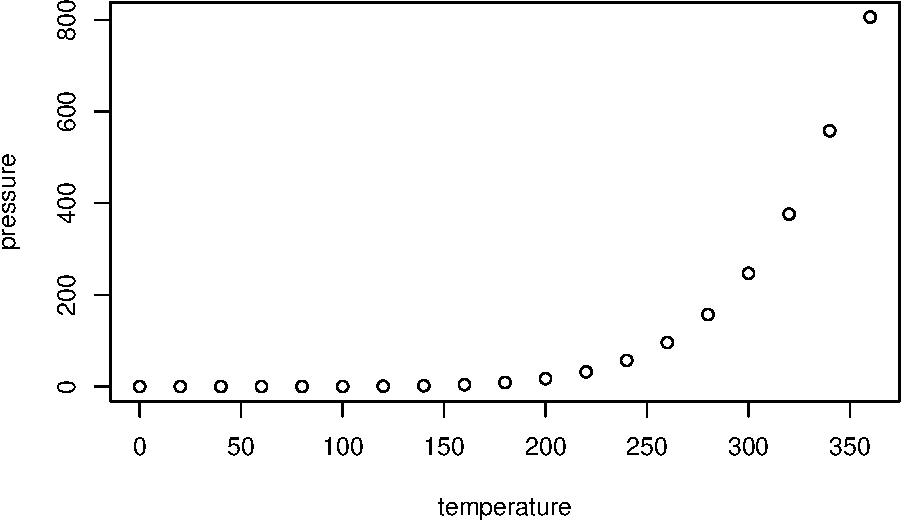
\includegraphics{StudentGoals_files/figure-latex/pressure-1.pdf}

Note that the \texttt{echo\ =\ FALSE} parameter was added to the code
chunk to prevent printing of the R code that generated the plot.

\begin{Shaded}
\begin{Highlighting}[]
\KeywordTok{library}\NormalTok{(tidyverse)}
\end{Highlighting}
\end{Shaded}

\begin{verbatim}
## -- Attaching packages ----------------------------------------------------------------------------------------------- tidyverse 1.2.1 --
\end{verbatim}

\begin{verbatim}
## v ggplot2 3.2.1     v purrr   0.3.3
## v tibble  2.1.3     v dplyr   0.8.3
## v tidyr   1.0.0     v stringr 1.4.0
## v readr   1.3.1     v forcats 0.4.0
\end{verbatim}

\begin{verbatim}
## -- Conflicts -------------------------------------------------------------------------------------------------- tidyverse_conflicts() --
## x dplyr::filter() masks stats::filter()
## x dplyr::lag()    masks stats::lag()
\end{verbatim}

\begin{Shaded}
\begin{Highlighting}[]
\KeywordTok{library}\NormalTok{(modelr)}
\KeywordTok{library}\NormalTok{(rsample)}
\KeywordTok{library}\NormalTok{(broom)}
\end{Highlighting}
\end{Shaded}

\begin{verbatim}
## 
## Attaching package: 'broom'
\end{verbatim}

\begin{verbatim}
## The following object is masked from 'package:modelr':
## 
##     bootstrap
\end{verbatim}

\begin{Shaded}
\begin{Highlighting}[]
\KeywordTok{library}\NormalTok{(magrittr)}
\end{Highlighting}
\end{Shaded}

\begin{verbatim}
## 
## Attaching package: 'magrittr'
\end{verbatim}

\begin{verbatim}
## The following object is masked from 'package:purrr':
## 
##     set_names
\end{verbatim}

\begin{verbatim}
## The following object is masked from 'package:tidyr':
## 
##     extract
\end{verbatim}

\begin{Shaded}
\begin{Highlighting}[]
\CommentTok{# set seed for randomization to ensure that results are always reproduced precisely}
\KeywordTok{set.seed}\NormalTok{(}\DecValTok{1234}\NormalTok{)}
\end{Highlighting}
\end{Shaded}

\begin{Shaded}
\begin{Highlighting}[]
\CommentTok{# read csv file (worse variable recognition)}
\NormalTok{f <-}\StringTok{ "data/StudentGoalsData.csv"}
\NormalTok{StudentGoalsData <-}\StringTok{ }\KeywordTok{read_csv}\NormalTok{(f)}
\end{Highlighting}
\end{Shaded}

\begin{verbatim}
## Parsed with column specification:
## cols(
##   .default = col_double()
## )
\end{verbatim}

\begin{verbatim}
## See spec(...) for full column specifications.
\end{verbatim}

\begin{Shaded}
\begin{Highlighting}[]
\CommentTok{# drop 'seq' column since it doesn't serve any purpose}
\NormalTok{StudentGoalsData <-}\StringTok{ }\NormalTok{StudentGoalsData  }\OperatorTok\StringTok{  }\NormalTok{ungroup  }\OperatorTok\StringTok{  }\KeywordTok{select}\NormalTok{(}\OperatorTok{-}\NormalTok{seq)}
\end{Highlighting}
\end{Shaded}

\begin{Shaded}
\begin{Highlighting}[]
\CommentTok{# count all the students before cleaning and dropping the data}
\NormalTok{n <-}\StringTok{ }\KeywordTok{tally}\NormalTok{(StudentGoalsData)}
\end{Highlighting}
\end{Shaded}

\begin{Shaded}
\begin{Highlighting}[]
\CommentTok{# # clean data - drop results contaiting empty cells}
\NormalTok{CleanedStudentGoalsData <-}\StringTok{ }\KeywordTok{drop_na}\NormalTok{(StudentGoalsData)}
\end{Highlighting}
\end{Shaded}

\begin{Shaded}
\begin{Highlighting}[]
\CommentTok{# save CleanedStudentGoalsData table in a simple variable called 'dat'}
\NormalTok{dat <-}\StringTok{ }\NormalTok{CleanedStudentGoalsData}
\end{Highlighting}
\end{Shaded}

\begin{Shaded}
\begin{Highlighting}[]
\CommentTok{# save CleanedStudentGoalsData table as tibble table in a variable called 'dat_tibble'}
\NormalTok{dat_tibble <-}\StringTok{ }\NormalTok{tibble}\OperatorTok{::}\KeywordTok{as_tibble}\NormalTok{(CleanedStudentGoalsData)}
\end{Highlighting}
\end{Shaded}

\begin{Shaded}
\begin{Highlighting}[]
\CommentTok{# Renaming columns according to random order: 6, 12, 11, 1, 7, 2, 10, 8, 5, 3, 9, 4}
\NormalTok{renamed_data <-}\StringTok{ }\NormalTok{dat_tibble }\OperatorTok
\StringTok{  }\KeywordTok{rename}\NormalTok{(}
    \DataTypeTok{Q6 =}\NormalTok{ q1,}
    \DataTypeTok{Q12 =}\NormalTok{ q2,}
    \DataTypeTok{Q11 =}\NormalTok{ q3,}
    \DataTypeTok{Q1 =}\NormalTok{ q4, }
    \DataTypeTok{Q7 =}\NormalTok{ q5, }
    \DataTypeTok{Q2 =}\NormalTok{ q6, }
    \DataTypeTok{Q10 =}\NormalTok{ q7, }
    \DataTypeTok{Q8 =}\NormalTok{ q8, }
    \DataTypeTok{Q5 =}\NormalTok{ q9, }
    \DataTypeTok{Q3 =}\NormalTok{ q10, }
    \DataTypeTok{Q9 =}\NormalTok{ q11, }
    \DataTypeTok{Q4 =}\NormalTok{ q12}
\NormalTok{  )}
\CommentTok{# going back to lower case 'q' to keep naming consistent with the original data set}
\NormalTok{renamed_data2 <-}\StringTok{ }\NormalTok{renamed_data }\OperatorTok
\StringTok{  }\KeywordTok{rename}\NormalTok{(}
    \DataTypeTok{q1 =}\NormalTok{ Q1, }\DataTypeTok{q2 =}\NormalTok{ Q2, }\DataTypeTok{q3 =}\NormalTok{ Q3, }\DataTypeTok{q4 =}\NormalTok{ Q4, }\DataTypeTok{q5 =}\NormalTok{ Q5, }\DataTypeTok{q6 =}\NormalTok{ Q6, }
    \DataTypeTok{q7 =}\NormalTok{ Q7, }\DataTypeTok{q8 =}\NormalTok{ Q8, }\DataTypeTok{q9 =}\NormalTok{ Q9, }\DataTypeTok{q10 =}\NormalTok{ Q10, }\DataTypeTok{q11=}\NormalTok{ Q11, }\DataTypeTok{q12 =}\NormalTok{ Q12}
\NormalTok{  )}
\CommentTok{# save renamed table in 'dat' variable}
\NormalTok{dat <-}\StringTok{ }\NormalTok{renamed_data2}
\end{Highlighting}
\end{Shaded}

\begin{Shaded}
\begin{Highlighting}[]
\CommentTok{# renaming values to their proper labeling from assets/'Student Goals - Coding Information.pdf'}
\CommentTok{# replace numericals in the 'sex' column with proper sex names}
\NormalTok{dat}\OperatorTok{$}\NormalTok{sex[dat}\OperatorTok{$}\NormalTok{sex}\OperatorTok{==}\DecValTok{1}\NormalTok{] <-}\StringTok{ 'Male'}
\NormalTok{dat}\OperatorTok{$}\NormalTok{sex[dat}\OperatorTok{$}\NormalTok{sex}\OperatorTok{==}\DecValTok{2}\NormalTok{] <-}\StringTok{ 'Female'}
\CommentTok{# replace numericals in the 'subject' column with proper subject names}
\NormalTok{dat}\OperatorTok{$}\NormalTok{subject[dat}\OperatorTok{$}\NormalTok{subject}\OperatorTok{==}\DecValTok{1}\NormalTok{] <-}\StringTok{ 'Management'}
\NormalTok{dat}\OperatorTok{$}\NormalTok{subject[dat}\OperatorTok{$}\NormalTok{subject}\OperatorTok{==}\DecValTok{2}\NormalTok{] <-}\StringTok{ 'Law'}
\NormalTok{dat}\OperatorTok{$}\NormalTok{subject[dat}\OperatorTok{$}\NormalTok{subject}\OperatorTok{==}\DecValTok{3}\NormalTok{] <-}\StringTok{ 'Tourism'}
\NormalTok{dat}\OperatorTok{$}\NormalTok{subject[dat}\OperatorTok{$}\NormalTok{subject}\OperatorTok{==}\DecValTok{4}\NormalTok{] <-}\StringTok{ 'General Economics'}
\NormalTok{dat}\OperatorTok{$}\NormalTok{subject[dat}\OperatorTok{$}\NormalTok{subject}\OperatorTok{==}\DecValTok{5}\NormalTok{] <-}\StringTok{ 'Accounting'}
\NormalTok{dat}\OperatorTok{$}\NormalTok{subject[dat}\OperatorTok{$}\NormalTok{subject}\OperatorTok{==}\DecValTok{6}\NormalTok{] <-}\StringTok{ 'Statistics'}
\end{Highlighting}
\end{Shaded}

\begin{Shaded}
\begin{Highlighting}[]
\CommentTok{## DATA EXPLORATION ##################################################################}
\CommentTok{# bar chart example}
\KeywordTok{ggplot}\NormalTok{(}\DataTypeTok{data =}\NormalTok{ diamonds) }\OperatorTok{+}\StringTok{ }
\StringTok{  }\KeywordTok{geom_bar}\NormalTok{(}\DataTypeTok{mapping =} \KeywordTok{aes}\NormalTok{(}\DataTypeTok{x =}\NormalTok{ cut))}
\end{Highlighting}
\end{Shaded}

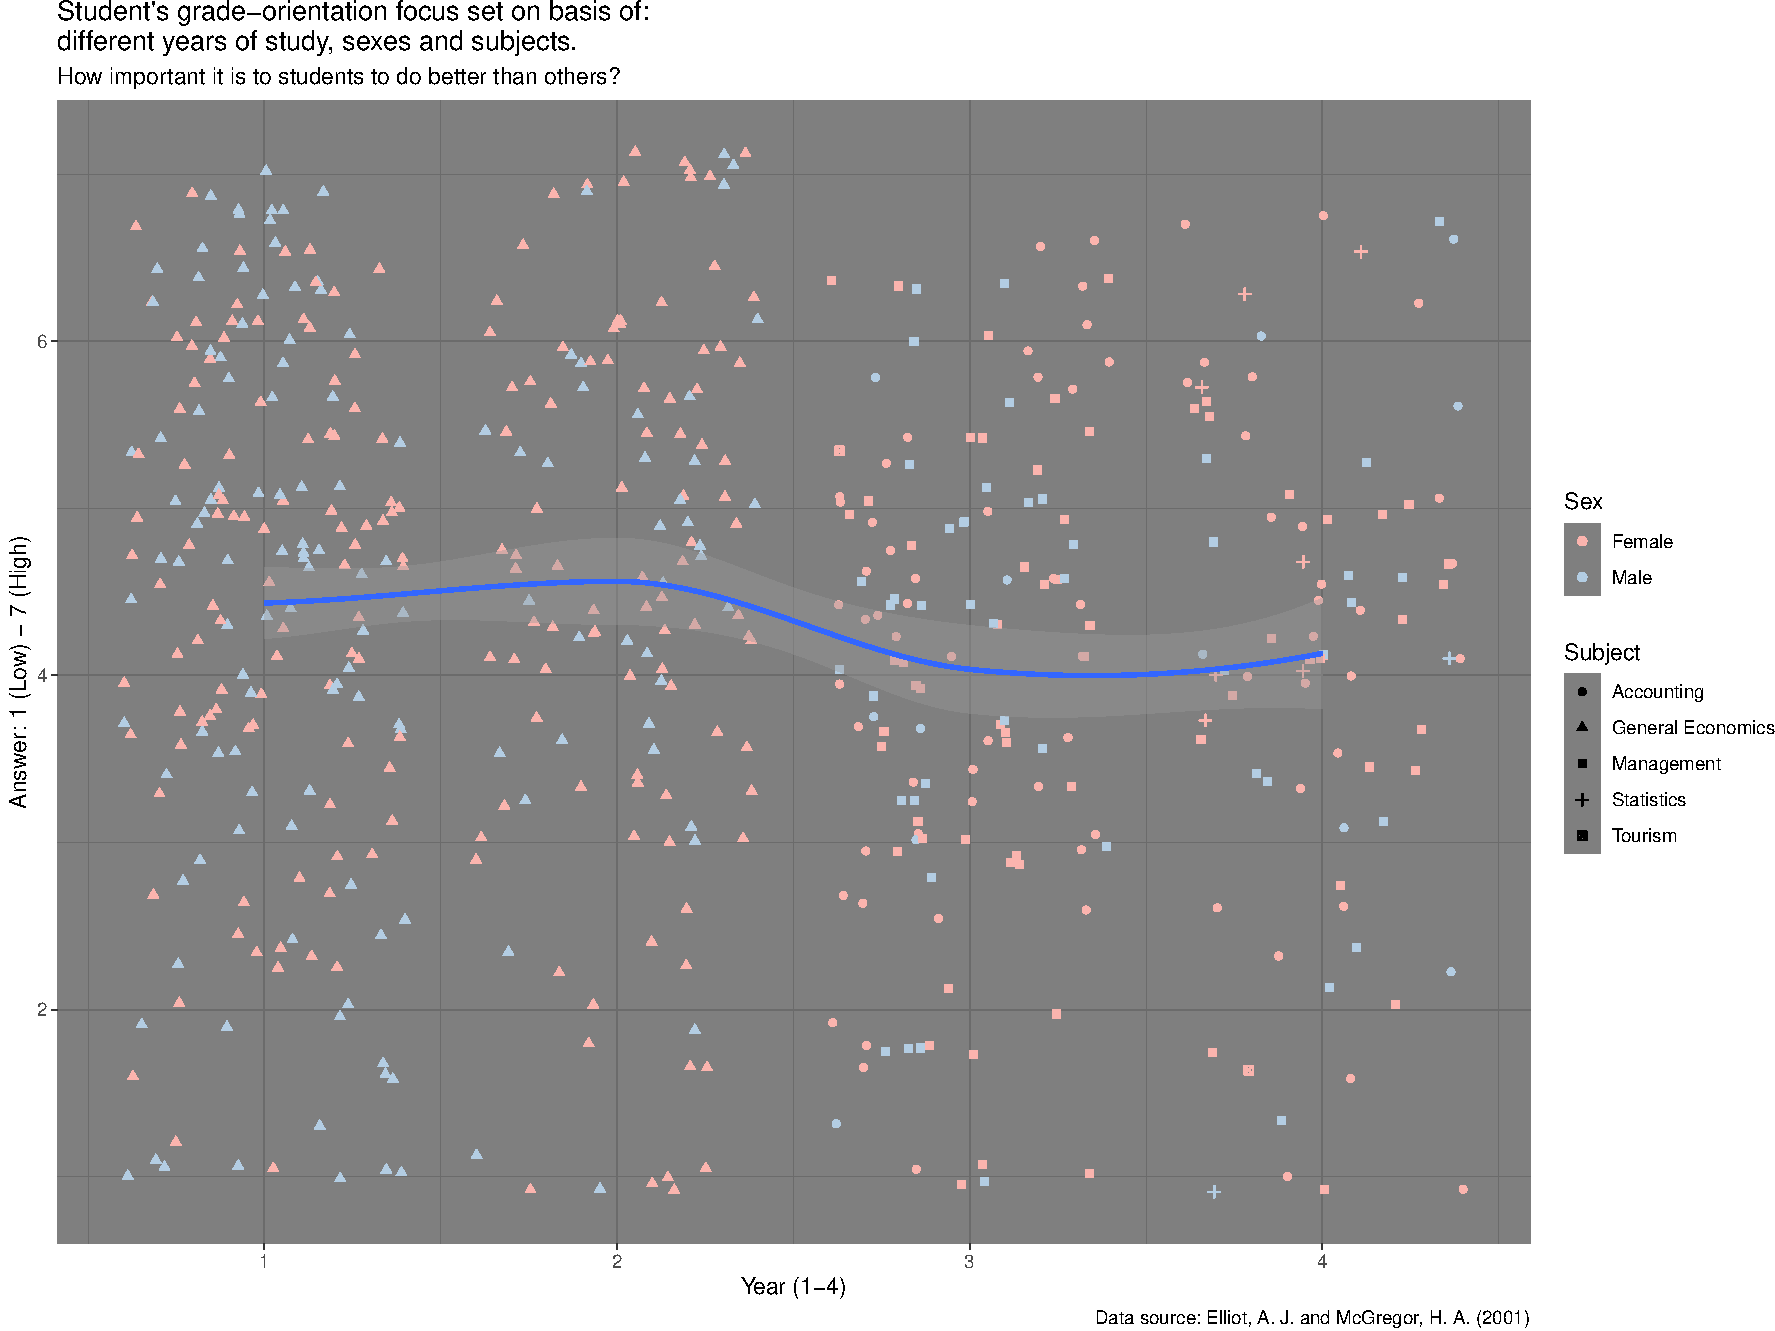
\includegraphics{StudentGoals_files/figure-latex/unnamed-chunk-11-1.pdf}

\begin{Shaded}
\begin{Highlighting}[]
\KeywordTok{head}\NormalTok{(diamonds)}
\end{Highlighting}
\end{Shaded}

\begin{longtable}[]{@{}rlllrrrrrr@{}}
\toprule
carat & cut & color & clarity & depth & table & price & x & y &
z\tabularnewline
\midrule
\endhead
0.23 & Ideal & E & SI2 & 61.5 & 55 & 326 & 3.95 & 3.98 &
2.43\tabularnewline
0.21 & Premium & E & SI1 & 59.8 & 61 & 326 & 3.89 & 3.84 &
2.31\tabularnewline
0.23 & Good & E & VS1 & 56.9 & 65 & 327 & 4.05 & 4.07 &
2.31\tabularnewline
0.29 & Premium & I & VS2 & 62.4 & 58 & 334 & 4.20 & 4.23 &
2.63\tabularnewline
0.31 & Good & J & SI2 & 63.3 & 58 & 335 & 4.34 & 4.35 &
2.75\tabularnewline
0.24 & Very Good & J & VVS2 & 62.8 & 57 & 336 & 3.94 & 3.96 &
2.48\tabularnewline
\bottomrule
\end{longtable}

\begin{Shaded}
\begin{Highlighting}[]
\KeywordTok{head}\NormalTok{(dat)}
\end{Highlighting}
\end{Shaded}

\begin{longtable}[]{@{}rrllrrrrrrrrrrrrrrr@{}}
\toprule
year & age & sex & subject & q6 & q12 & q11 & q1 & q7 & q2 & q10 & q8 &
q5 & q3 & q9 & q4 & interest & enjoy & mastgrad\tabularnewline
\midrule
\endhead
4 & 20 & Male & Management & 6 & 2 & 4 & 6 & 7 & 5 & 4 & 5 & 1 & 3 & 6 &
6 & 7 & 5 & 2\tabularnewline
4 & 20 & Male & Management & 3 & 1 & 1 & 3 & 5 & 3 & 4 & 5 & 3 & 1 & 5 &
1 & 7 & 7 & 5\tabularnewline
3 & 19 & Female & Management & 2 & 2 & 1 & 6 & 5 & 4 & 1 & 7 & 1 & 1 & 5
& 1 & 7 & 7 & 4\tabularnewline
3 & 19 & Male & Management & 4 & 5 & 5 & 3 & 6 & 4 & 6 & 6 & 4 & 4 & 6 &
3 & 7 & 6 & 3\tabularnewline
3 & 18 & Female & Management & 6 & 4 & 2 & 4 & 7 & 4 & 6 & 7 & 2 & 2 & 7
& 2 & 7 & 7 & 1\tabularnewline
3 & 19 & Male & Management & 7 & 2 & 2 & 6 & 7 & 6 & 7 & 7 & 5 & 5 & 7 &
5 & 7 & 7 & 1\tabularnewline
\bottomrule
\end{longtable}

\begin{Shaded}
\begin{Highlighting}[]
\CommentTok{#bar chart example 2}
\KeywordTok{ggplot}\NormalTok{(}\DataTypeTok{data =}\NormalTok{ diamonds) }\OperatorTok{+}\StringTok{ }
\StringTok{  }\KeywordTok{geom_bar}\NormalTok{(}\DataTypeTok{mapping =} \KeywordTok{aes}\NormalTok{(}\DataTypeTok{x =}\NormalTok{ cut, }\DataTypeTok{fill =}\NormalTok{ clarity))}
\end{Highlighting}
\end{Shaded}

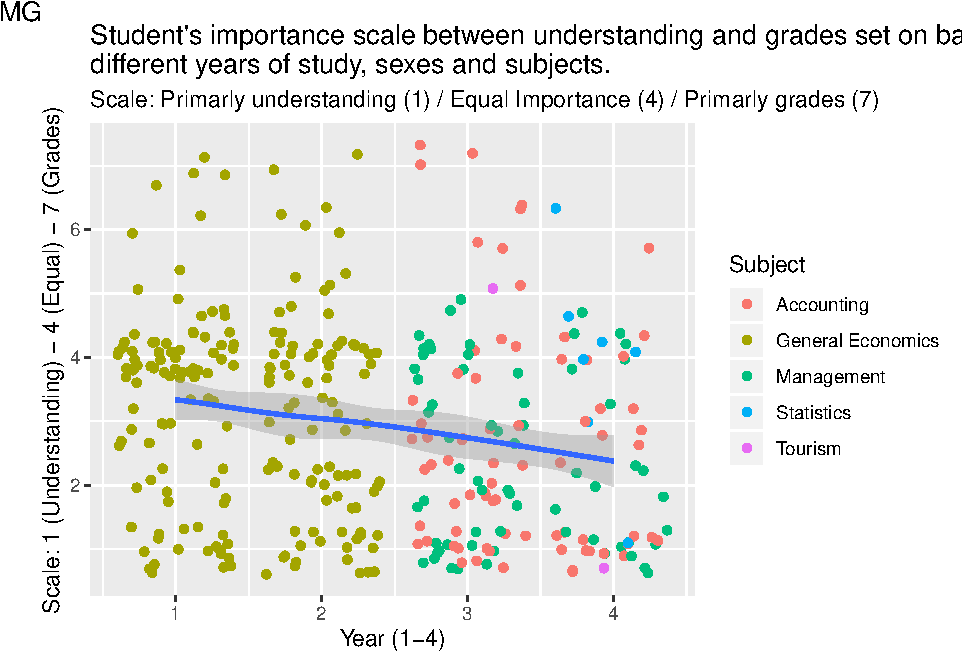
\includegraphics{StudentGoals_files/figure-latex/unnamed-chunk-11-2.pdf}

\begin{Shaded}
\begin{Highlighting}[]
\CommentTok{# gender in numbers}
\KeywordTok{ggplot}\NormalTok{(}\DataTypeTok{data =}\NormalTok{ dat) }\OperatorTok{+}\StringTok{ }
\StringTok{  }\KeywordTok{geom_bar}\NormalTok{(}\DataTypeTok{mapping =} \KeywordTok{aes}\NormalTok{(}\DataTypeTok{x =}\NormalTok{ sex, }\DataTypeTok{fill =}\NormalTok{ sex))}
\end{Highlighting}
\end{Shaded}

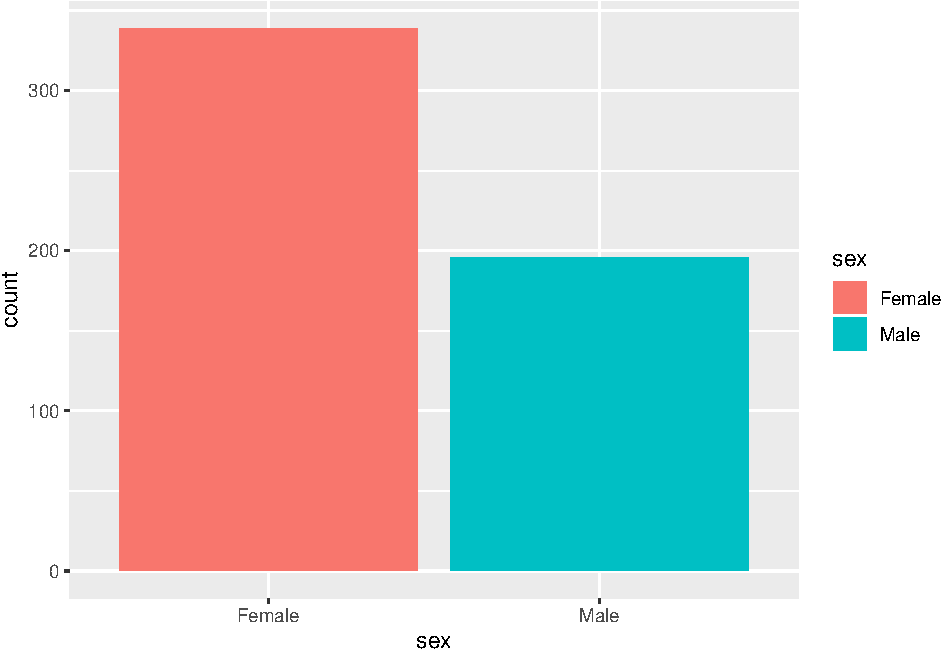
\includegraphics{StudentGoals_files/figure-latex/unnamed-chunk-11-3.pdf}

\begin{Shaded}
\begin{Highlighting}[]
\CommentTok{# subject by gender}
\KeywordTok{ggplot}\NormalTok{(}\DataTypeTok{data =}\NormalTok{ dat) }\OperatorTok{+}\StringTok{ }
\StringTok{  }\KeywordTok{geom_bar}\NormalTok{(}\DataTypeTok{mapping =} \KeywordTok{aes}\NormalTok{(}\DataTypeTok{x =}\NormalTok{ sex, }\DataTypeTok{fill =}\NormalTok{ subject))}
\end{Highlighting}
\end{Shaded}

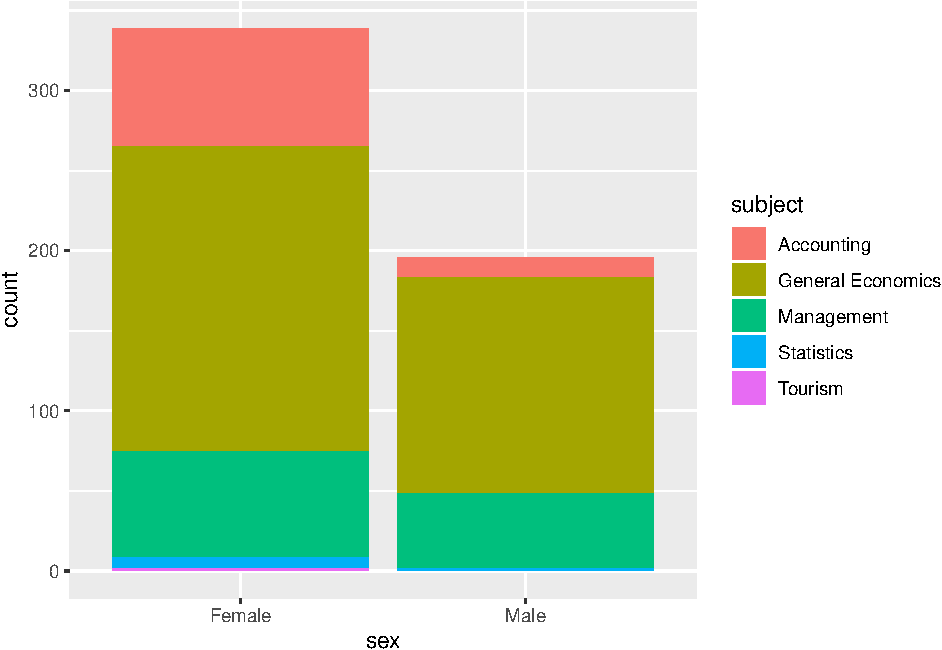
\includegraphics{StudentGoals_files/figure-latex/unnamed-chunk-11-4.pdf}

\begin{Shaded}
\begin{Highlighting}[]
\CommentTok{#subject by gender with alpha blending}
\KeywordTok{ggplot}\NormalTok{(}\DataTypeTok{data =}\NormalTok{ dat) }\OperatorTok{+}\StringTok{ }
\StringTok{  }\KeywordTok{geom_bar}\NormalTok{(}\DataTypeTok{alpha =} \FloatTok{0.85}\NormalTok{, }\DataTypeTok{mapping =} \KeywordTok{aes}\NormalTok{(}\DataTypeTok{x =}\NormalTok{ sex, }\DataTypeTok{fill =}\NormalTok{ subject))}
\end{Highlighting}
\end{Shaded}

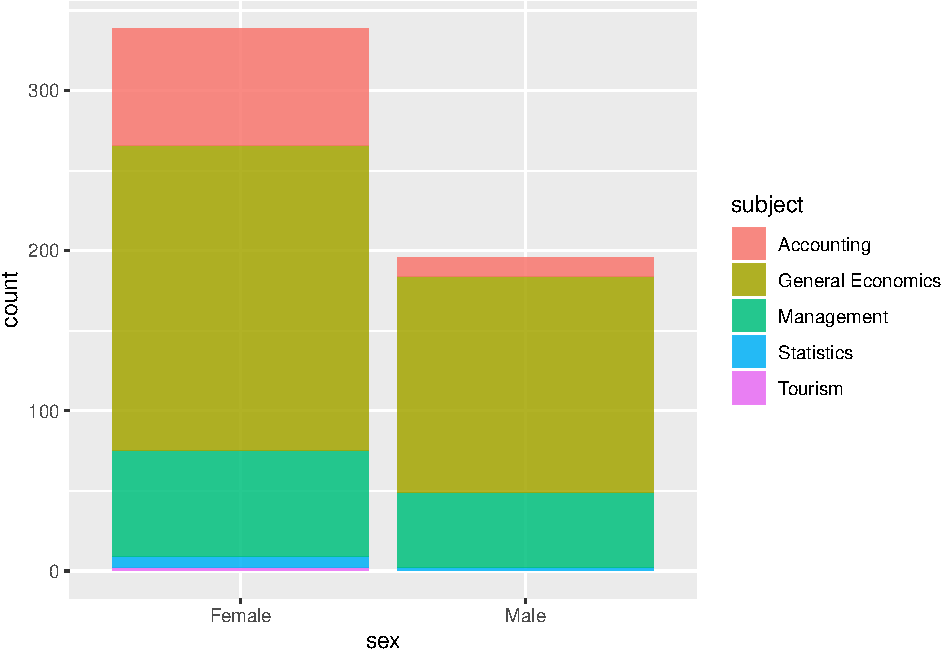
\includegraphics{StudentGoals_files/figure-latex/unnamed-chunk-11-5.pdf}

\begin{Shaded}
\begin{Highlighting}[]
\CommentTok{#subject by gender and normalizing using position = "fill"}
\KeywordTok{ggplot}\NormalTok{(}\DataTypeTok{data =}\NormalTok{ dat) }\OperatorTok{+}\StringTok{ }
\StringTok{  }\KeywordTok{geom_bar}\NormalTok{(}\DataTypeTok{mapping =} \KeywordTok{aes}\NormalTok{(}\DataTypeTok{x =}\NormalTok{ sex, }\DataTypeTok{fill =}\NormalTok{ subject), }\DataTypeTok{position =} \StringTok{"fill"}\NormalTok{)}
\end{Highlighting}
\end{Shaded}

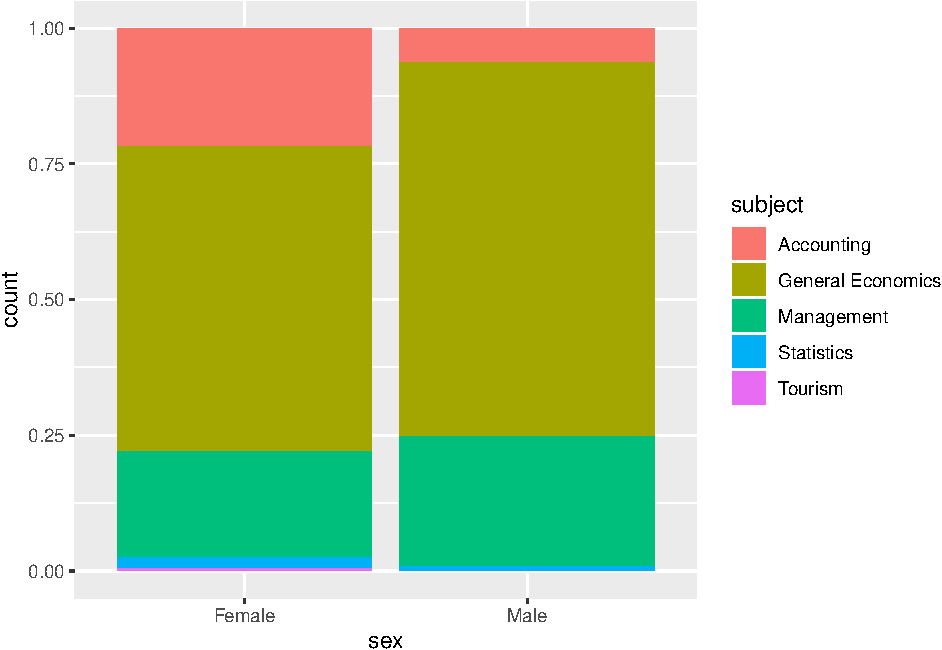
\includegraphics{StudentGoals_files/figure-latex/unnamed-chunk-11-6.pdf}

\begin{Shaded}
\begin{Highlighting}[]
\CommentTok{#subject by gender and normalizing using position = "dodge" to place overlapping objects directly beside one another}
\KeywordTok{ggplot}\NormalTok{(}\DataTypeTok{data =}\NormalTok{ dat) }\OperatorTok{+}\StringTok{ }
\StringTok{  }\KeywordTok{geom_bar}\NormalTok{(}\DataTypeTok{mapping =} \KeywordTok{aes}\NormalTok{(}\DataTypeTok{x =}\NormalTok{ sex, }\DataTypeTok{fill =}\NormalTok{ subject), }\DataTypeTok{position =} \StringTok{"dodge"}\NormalTok{)}
\end{Highlighting}
\end{Shaded}

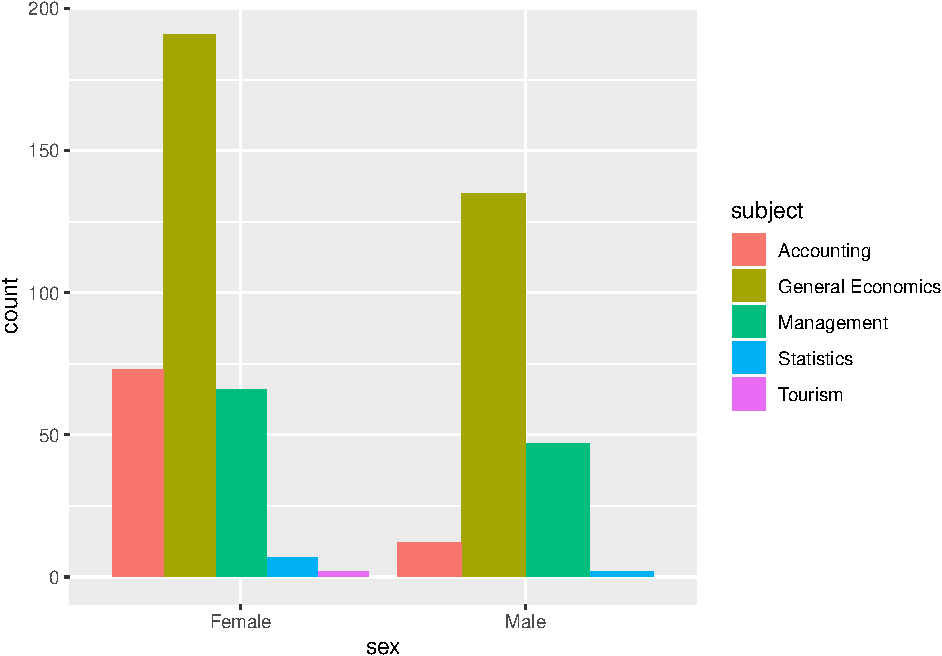
\includegraphics{StudentGoals_files/figure-latex/unnamed-chunk-11-7.pdf}

\begin{Shaded}
\begin{Highlighting}[]
\CommentTok{# age by gender}
\KeywordTok{ggplot}\NormalTok{(}\DataTypeTok{data =}\NormalTok{ dat) }\OperatorTok{+}\StringTok{ }
\StringTok{  }\KeywordTok{geom_bar}\NormalTok{(}\DataTypeTok{mapping =} \KeywordTok{aes}\NormalTok{(}\DataTypeTok{x =}\NormalTok{ age, }\DataTypeTok{fill =}\NormalTok{ sex))}
\end{Highlighting}
\end{Shaded}

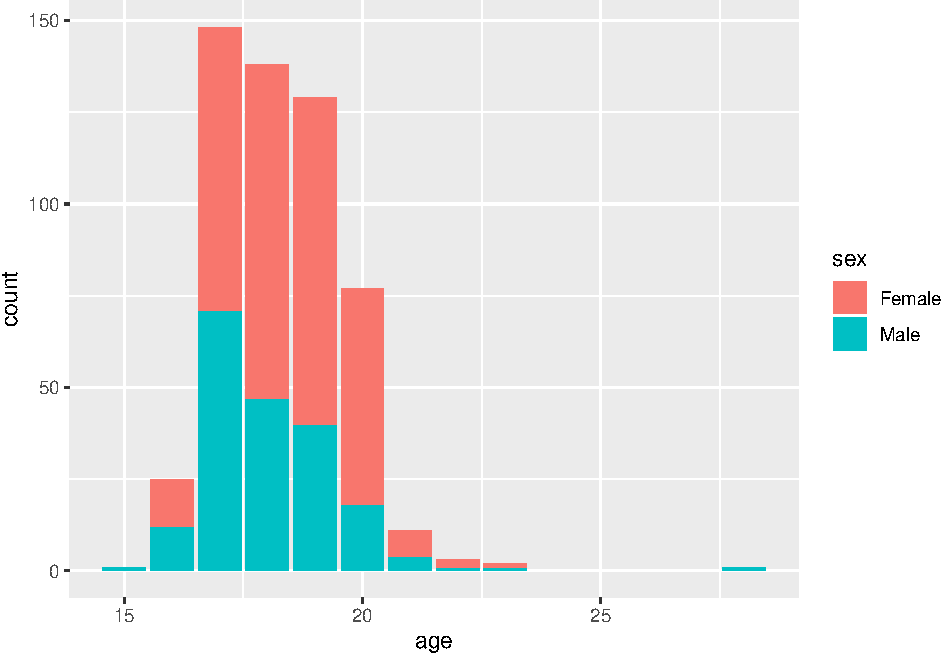
\includegraphics{StudentGoals_files/figure-latex/unnamed-chunk-11-8.pdf}

\begin{Shaded}
\begin{Highlighting}[]
\CommentTok{# age by subject}
\KeywordTok{ggplot}\NormalTok{(}\DataTypeTok{data =}\NormalTok{ dat) }\OperatorTok{+}\StringTok{ }
\StringTok{  }\KeywordTok{geom_bar}\NormalTok{(}\DataTypeTok{mapping =} \KeywordTok{aes}\NormalTok{(}\DataTypeTok{x =}\NormalTok{ age, }\DataTypeTok{fill =}\NormalTok{ subject))}
\end{Highlighting}
\end{Shaded}

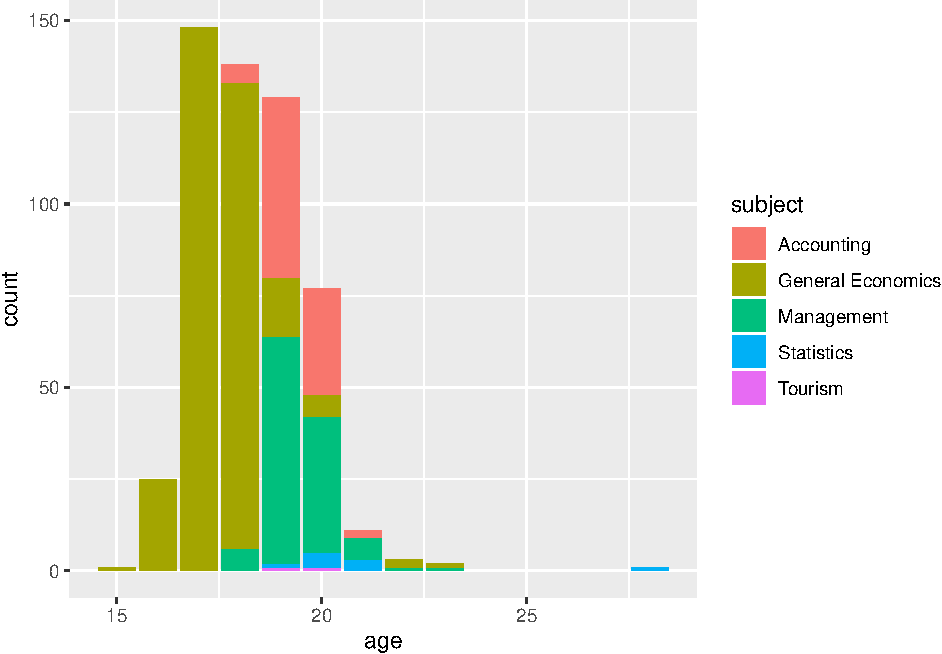
\includegraphics{StudentGoals_files/figure-latex/unnamed-chunk-11-9.pdf}

\begin{Shaded}
\begin{Highlighting}[]
\CommentTok{# course year by gender}
\KeywordTok{ggplot}\NormalTok{(}\DataTypeTok{data =}\NormalTok{ dat) }\OperatorTok{+}\StringTok{ }
\StringTok{  }\KeywordTok{geom_bar}\NormalTok{(}\DataTypeTok{mapping =} \KeywordTok{aes}\NormalTok{(}\DataTypeTok{x =}\NormalTok{ year, }\DataTypeTok{fill =}\NormalTok{ sex))}
\end{Highlighting}
\end{Shaded}

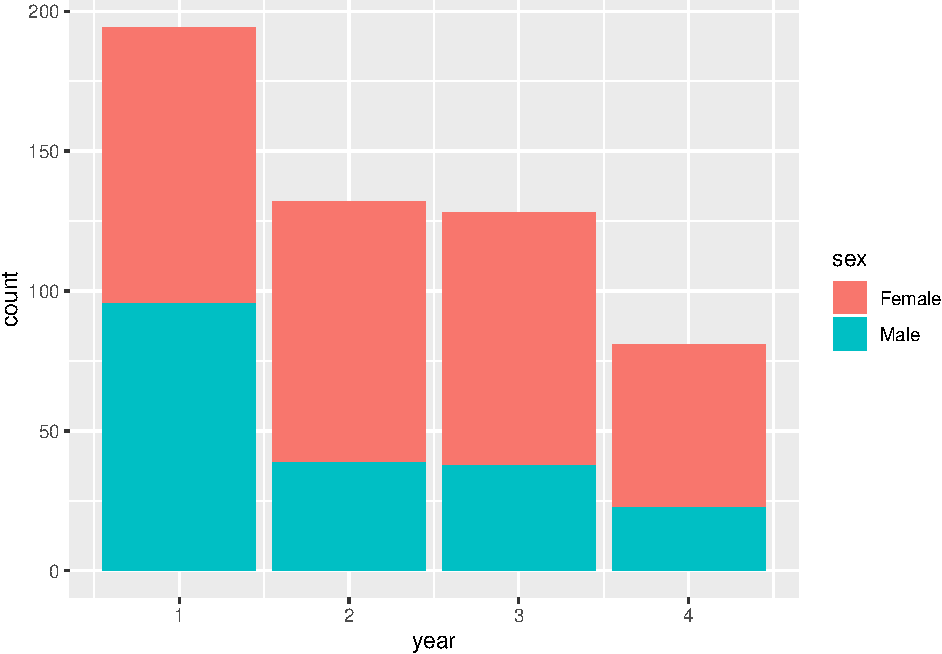
\includegraphics{StudentGoals_files/figure-latex/unnamed-chunk-11-10.pdf}

\begin{Shaded}
\begin{Highlighting}[]
\CommentTok{# "expect my courses this semester to be very interesting" by gender}
\KeywordTok{ggplot}\NormalTok{(}\DataTypeTok{data =}\NormalTok{ dat) }\OperatorTok{+}\StringTok{ }
\StringTok{  }\KeywordTok{geom_bar}\NormalTok{(}\DataTypeTok{mapping =} \KeywordTok{aes}\NormalTok{(}\DataTypeTok{x =}\NormalTok{ interest, }\DataTypeTok{fill =}\NormalTok{ sex))}
\end{Highlighting}
\end{Shaded}

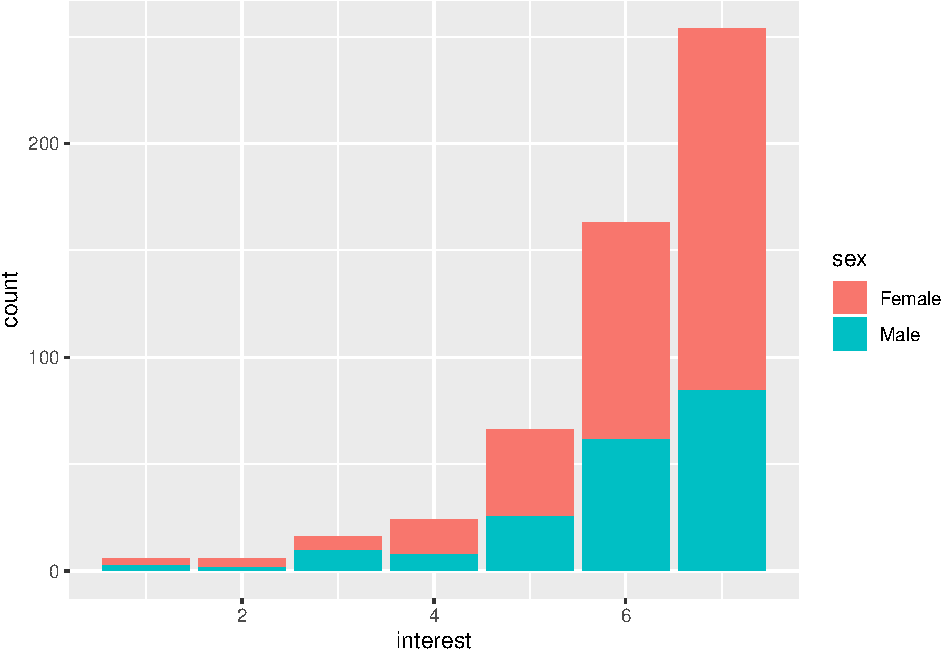
\includegraphics{StudentGoals_files/figure-latex/unnamed-chunk-11-11.pdf}

\begin{Shaded}
\begin{Highlighting}[]
\CommentTok{# "expect my courses this semester to be very enjoyable" by gender}
\KeywordTok{ggplot}\NormalTok{(}\DataTypeTok{data =}\NormalTok{ dat) }\OperatorTok{+}\StringTok{ }
\StringTok{  }\KeywordTok{geom_bar}\NormalTok{(}\DataTypeTok{mapping =} \KeywordTok{aes}\NormalTok{(}\DataTypeTok{x =}\NormalTok{ enjoy, }\DataTypeTok{fill =}\NormalTok{ sex))}
\end{Highlighting}
\end{Shaded}

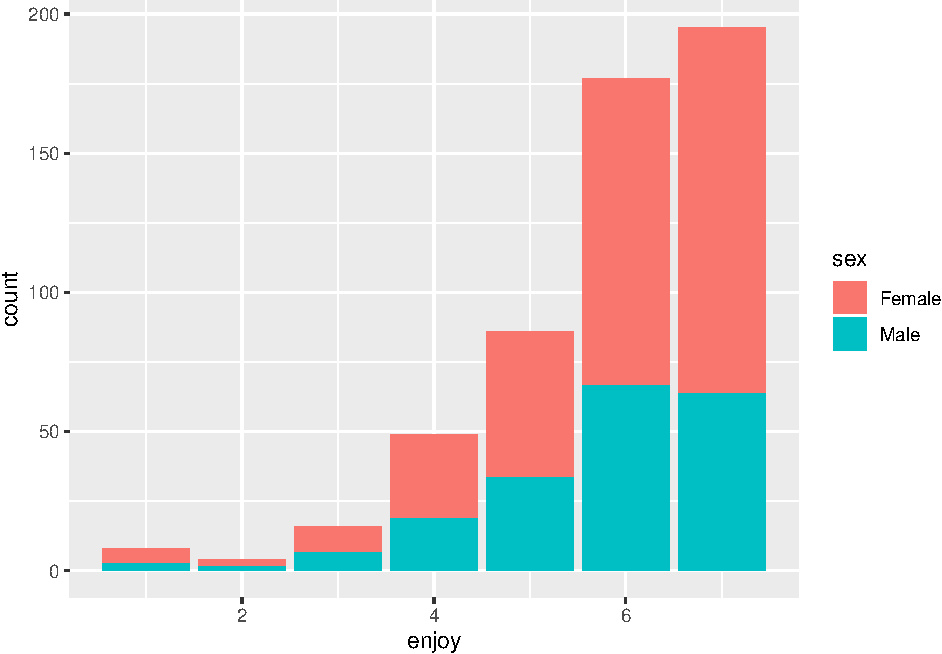
\includegraphics{StudentGoals_files/figure-latex/unnamed-chunk-11-12.pdf}

\begin{Shaded}
\begin{Highlighting}[]
\CommentTok{# relative importance by gender}
\KeywordTok{ggplot}\NormalTok{(}\DataTypeTok{data =}\NormalTok{ dat) }\OperatorTok{+}\StringTok{ }
\StringTok{  }\KeywordTok{geom_bar}\NormalTok{(}\DataTypeTok{mapping =} \KeywordTok{aes}\NormalTok{(}\DataTypeTok{x =}\NormalTok{ mastgrad, }\DataTypeTok{fill =}\NormalTok{ sex))}
\end{Highlighting}
\end{Shaded}

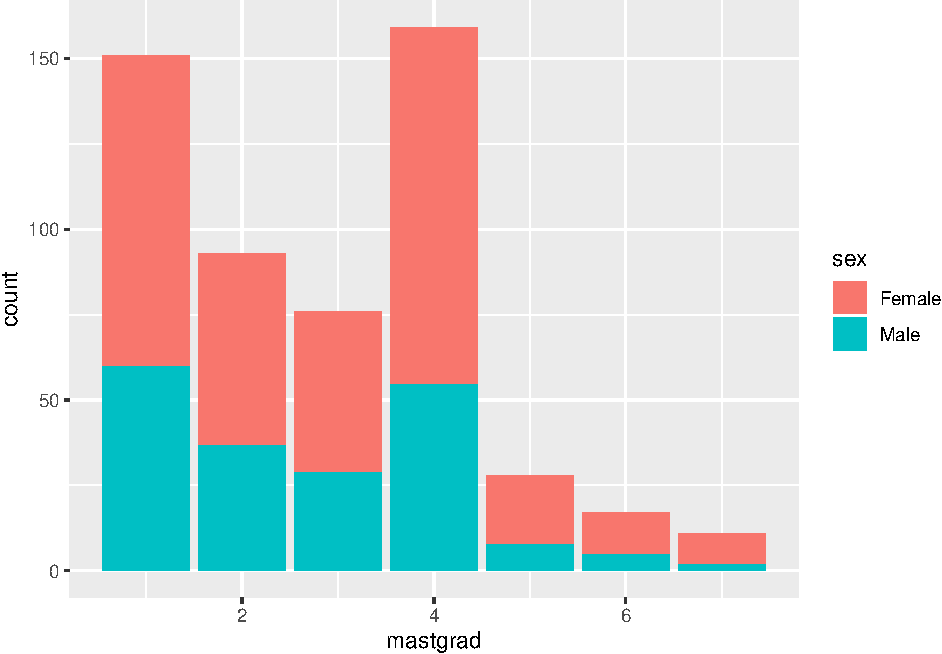
\includegraphics{StudentGoals_files/figure-latex/unnamed-chunk-11-13.pdf}

\begin{Shaded}
\begin{Highlighting}[]
\CommentTok{#subject by gender and normalizing using position = "dodge" to place overlapping objects directly beside one another}
\KeywordTok{ggplot}\NormalTok{(}\DataTypeTok{data =}\NormalTok{ dat) }\OperatorTok{+}\StringTok{ }
\StringTok{  }\KeywordTok{geom_bar}\NormalTok{(}\DataTypeTok{mapping =} \KeywordTok{aes}\NormalTok{(}\DataTypeTok{x =}\NormalTok{ sex, }\DataTypeTok{fill =}\NormalTok{ subject), }\DataTypeTok{position =} \StringTok{"dodge"}\NormalTok{)}
\end{Highlighting}
\end{Shaded}

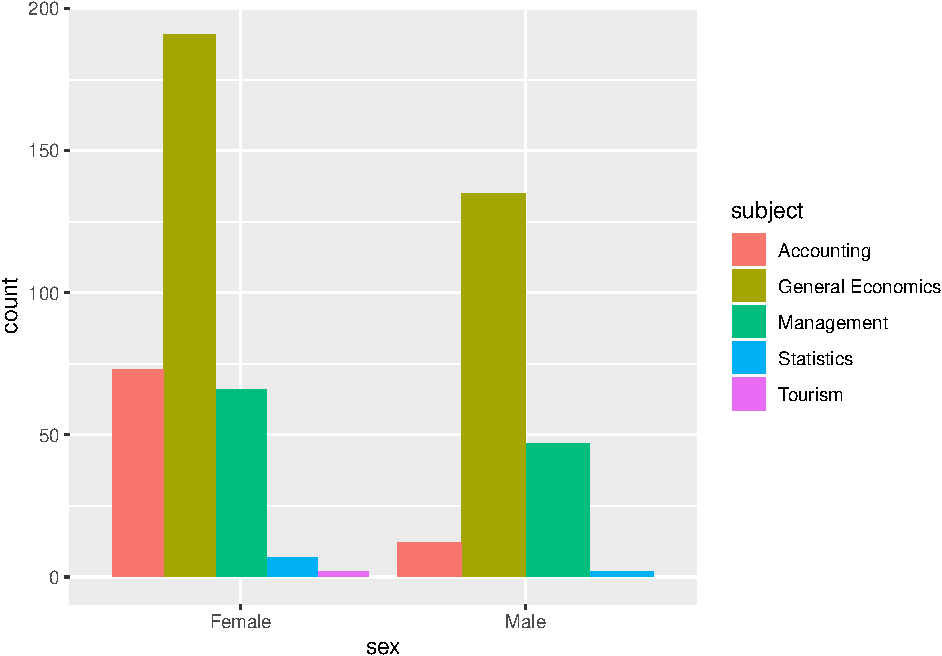
\includegraphics{StudentGoals_files/figure-latex/unnamed-chunk-11-14.pdf}

\begin{Shaded}
\begin{Highlighting}[]
\CommentTok{# plot answers to q1 with relation to the student's year}
\KeywordTok{ggplot}\NormalTok{(}\DataTypeTok{data =}\NormalTok{ dat) }\OperatorTok{+}\StringTok{ }
\StringTok{  }\KeywordTok{geom_point}\NormalTok{(}\DataTypeTok{mapping =} \KeywordTok{aes}\NormalTok{(}\DataTypeTok{x =}\NormalTok{ year, }\DataTypeTok{y =}\NormalTok{ q1, }\DataTypeTok{colour =}\NormalTok{ year))}
\end{Highlighting}
\end{Shaded}

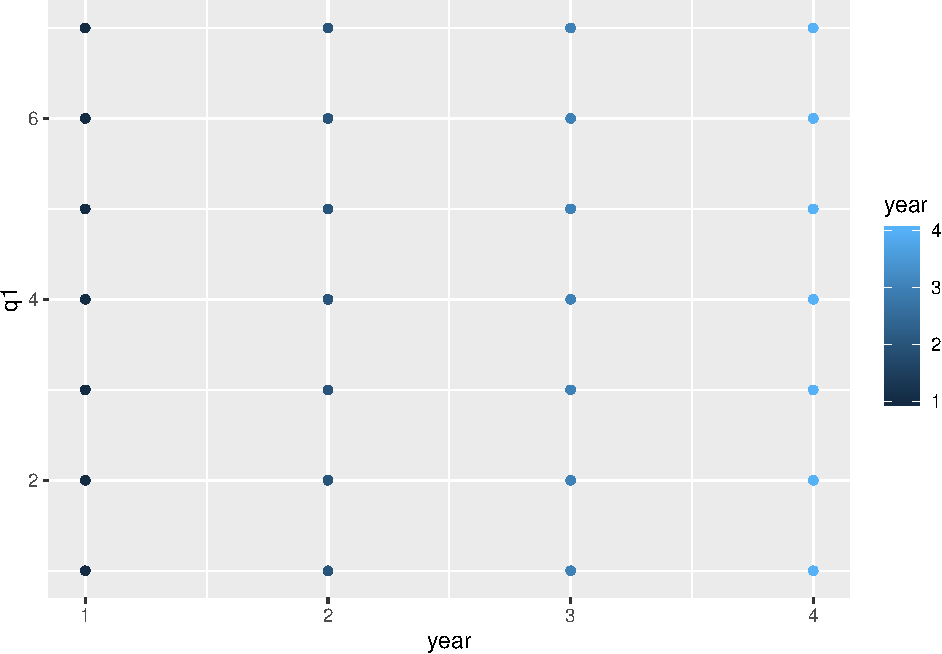
\includegraphics{StudentGoals_files/figure-latex/unnamed-chunk-11-15.pdf}

\begin{Shaded}
\begin{Highlighting}[]
\CommentTok{##############################################################################}
\end{Highlighting}
\end{Shaded}

\begin{Shaded}
\begin{Highlighting}[]
\CommentTok{## Calculate mean for 7 categories:}
\CommentTok{# across 7 categories:}
\CommentTok{# - q1, q2, q3 - Performance approach questions}
\CommentTok{# - q4, q5, q6 - Performance avoidance questions}
\CommentTok{# - q7, q8, q9 - Mastery-Approach}
\CommentTok{# - q10, q11, q12 - Mastery-Avoidance}
\CommentTok{# - Interest}
\CommentTok{# - Enjoyment}
\CommentTok{# - Understanding/Grades}

\NormalTok{mean_dat <-}\StringTok{ }\NormalTok{dat}
\CommentTok{# get mean from q1, q2, q3 columns (Performance approach questions) for all the students}
\CommentTok{# save the results in 'm1' colum and add it to 'mean_dat' table}
\NormalTok{mean_dat <-}\StringTok{ }\NormalTok{mean_dat }\OperatorTok\StringTok{ }
\StringTok{  }\KeywordTok{mutate}\NormalTok{(}\DataTypeTok{m1 =} \KeywordTok{pmap_dbl}\NormalTok{(}\KeywordTok{select}\NormalTok{(., }\KeywordTok{c}\NormalTok{(}\StringTok{"q1"}\NormalTok{, }\StringTok{"q2"}\NormalTok{, }\StringTok{"q3"}\NormalTok{)), }\ControlFlowTok{function}\NormalTok{(...) }\KeywordTok{mean}\NormalTok{(}\KeywordTok{c}\NormalTok{(...))))}

\CommentTok{# get mean from q4, q5, q6 columns (Performance avoidance questions) for all the students,}
\CommentTok{# save the results in 'm2' colum and add it to 'mean_dat' table}
\NormalTok{mean_dat <-}\StringTok{ }\NormalTok{mean_dat }\OperatorTok\StringTok{ }
\StringTok{  }\KeywordTok{mutate}\NormalTok{(}\DataTypeTok{m2 =} \KeywordTok{pmap_dbl}\NormalTok{(}\KeywordTok{select}\NormalTok{(., }\KeywordTok{c}\NormalTok{(}\StringTok{"q4"}\NormalTok{, }\StringTok{"q5"}\NormalTok{, }\StringTok{"q6"}\NormalTok{)), }\ControlFlowTok{function}\NormalTok{(...) }\KeywordTok{mean}\NormalTok{(}\KeywordTok{c}\NormalTok{(...))))}

\CommentTok{# get mean from q7, q8, q9 columns (Mastery approach questions) for all the students}
\CommentTok{# save the results in 'm3' colum and add it to 'mean_dat' table}
\NormalTok{mean_dat <-}\StringTok{ }\NormalTok{mean_dat }\OperatorTok\StringTok{ }
\StringTok{  }\KeywordTok{mutate}\NormalTok{(}\DataTypeTok{m3 =} \KeywordTok{pmap_dbl}\NormalTok{(}\KeywordTok{select}\NormalTok{(., }\KeywordTok{c}\NormalTok{(}\StringTok{"q7"}\NormalTok{, }\StringTok{"q8"}\NormalTok{, }\StringTok{"q9"}\NormalTok{)), }\ControlFlowTok{function}\NormalTok{(...) }\KeywordTok{mean}\NormalTok{(}\KeywordTok{c}\NormalTok{(...))))}

\CommentTok{# get mean from q10, q11, q12 columns (Mastery avoidance questions) for all the students }
\CommentTok{# save the results in 'm4' colum and add it to 'mean_dat' table}
\NormalTok{mean_dat <-}\StringTok{ }\NormalTok{mean_dat }\OperatorTok\StringTok{ }
\StringTok{  }\KeywordTok{mutate}\NormalTok{(}\DataTypeTok{m4 =} \KeywordTok{pmap_dbl}\NormalTok{(}\KeywordTok{select}\NormalTok{(., }\KeywordTok{c}\NormalTok{(}\StringTok{"q10"}\NormalTok{, }\StringTok{"q11"}\NormalTok{, }\StringTok{"q12"}\NormalTok{)), }\ControlFlowTok{function}\NormalTok{(...) }\KeywordTok{mean}\NormalTok{(}\KeywordTok{c}\NormalTok{(...))))}

\CommentTok{# get mean from 'interest' column (Course interestedness expectations) for all the students }
\CommentTok{# save the results in 'm_interest' colum and add it to 'mean_dat' table}
\NormalTok{mean_dat <-}\StringTok{ }\NormalTok{mean_dat }\OperatorTok\StringTok{ }
\StringTok{  }\KeywordTok{mutate}\NormalTok{(}\DataTypeTok{m_interest =} \KeywordTok{pmap_dbl}\NormalTok{(}\KeywordTok{select}\NormalTok{(., }\KeywordTok{c}\NormalTok{(}\StringTok{"interest"}\NormalTok{)), }\ControlFlowTok{function}\NormalTok{(...) }\KeywordTok{mean}\NormalTok{(}\KeywordTok{c}\NormalTok{(...))))}

\CommentTok{# get mean from 'enjoy' column (Course enjoyment expectations) for all the students }
\CommentTok{# save the results in 'm_interest' colum and add it to 'mean_dat' table}
\NormalTok{mean_dat <-}\StringTok{ }\NormalTok{mean_dat }\OperatorTok\StringTok{ }
\StringTok{  }\KeywordTok{mutate}\NormalTok{(}\DataTypeTok{m_enjoy =} \KeywordTok{pmap_dbl}\NormalTok{(}\KeywordTok{select}\NormalTok{(., }\KeywordTok{c}\NormalTok{(}\StringTok{"enjoy"}\NormalTok{)), }\ControlFlowTok{function}\NormalTok{(...) }\KeywordTok{mean}\NormalTok{(}\KeywordTok{c}\NormalTok{(...))))}

\CommentTok{# get mean from 'mastgrad' column (1 (Understanding) - 7 (Grades) Importance) for all the students }
\CommentTok{# save the results in 'm_interest' colum and add it to 'mean_dat' table}
\NormalTok{mean_dat <-}\StringTok{ }\NormalTok{mean_dat }\OperatorTok\StringTok{ }
\StringTok{  }\KeywordTok{mutate}\NormalTok{(}\DataTypeTok{m_mastgrad =} \KeywordTok{pmap_dbl}\NormalTok{(}\KeywordTok{select}\NormalTok{(., }\KeywordTok{c}\NormalTok{(}\StringTok{"mastgrad"}\NormalTok{)), }\ControlFlowTok{function}\NormalTok{(...) }\KeywordTok{mean}\NormalTok{(}\KeywordTok{c}\NormalTok{(...))))}

\CommentTok{# save final cleaned table}
\KeywordTok{write_csv}\NormalTok{(mean_dat, }\StringTok{"data/MeanCleanedStudentGoals.csv"}\NormalTok{)}
\CommentTok{# save final cleaned table as tibble table}
\NormalTok{dat_tibble <-}\StringTok{ }\KeywordTok{as_tibble}\NormalTok{(mean_dat)}
\end{Highlighting}
\end{Shaded}

\begin{Shaded}
\begin{Highlighting}[]
\CommentTok{# m1}
\CommentTok{# Plot mean results of performance approach questions}
\CommentTok{# for all students with relation to student's year, sex and subject}
\CommentTok{# data}
\NormalTok{d <-}\StringTok{ }\KeywordTok{ggplot}\NormalTok{(}\DataTypeTok{data =}\NormalTok{ dat, }\KeywordTok{aes}\NormalTok{(mean_dat}\OperatorTok{$}\NormalTok{year, mean_dat}\OperatorTok{$}\NormalTok{m1))}
\CommentTok{# mapping data (use "jitter" to improve the graph and avoid gridding)}
\NormalTok{l <-}\StringTok{ }\NormalTok{d }\OperatorTok{+}\StringTok{ }\KeywordTok{geom_jitter}\NormalTok{(}\KeywordTok{aes}\NormalTok{(}\DataTypeTok{colour =}\NormalTok{ sex, }\DataTypeTok{shape =}\NormalTok{ subject))}
\CommentTok{# smoothing}
\NormalTok{s <-}\StringTok{ }\NormalTok{l }\OperatorTok{+}\StringTok{ }\KeywordTok{geom_smooth}\NormalTok{(}\DataTypeTok{method =}\NormalTok{ loess, }\DataTypeTok{formula =}\NormalTok{ y }\OperatorTok{~}\StringTok{ }\NormalTok{x, }\DataTypeTok{se =} \OtherTok{TRUE}\NormalTok{)}
\CommentTok{# adding theme}
\NormalTok{t <-}\StringTok{ }\NormalTok{s }\OperatorTok{+}\StringTok{ }\KeywordTok{theme_dark}\NormalTok{()}
\CommentTok{# adding colouring}
\NormalTok{c <-}\StringTok{ }\NormalTok{t }\OperatorTok{+}\StringTok{ }\KeywordTok{scale_colour_brewer}\NormalTok{(}\DataTypeTok{palette =} \StringTok{"Pastel1"}\NormalTok{)}
\CommentTok{# adding labels}
\NormalTok{c }\OperatorTok{+}\StringTok{ }\KeywordTok{labs}\NormalTok{(}
  \DataTypeTok{title =} \StringTok{"Student's grade-orientation focus set on basis of:}
\StringTok{different years of study, sexes and subjects."}\NormalTok{,}
  \DataTypeTok{subtitle =} \StringTok{"How important it is to students to do better than others?"}\NormalTok{,}
  \DataTypeTok{caption =} \StringTok{"Data source: Elliot, A. J. and McGregor, H. A. (2001)"}\NormalTok{,}
  \DataTypeTok{x =} \StringTok{"Year (1-4)"}\NormalTok{,}
  \DataTypeTok{y =} \StringTok{"Answer: 1 (Low) - 7 (High)"}\NormalTok{,}
  \DataTypeTok{colour =} \StringTok{"Sex"}\NormalTok{,}
  \DataTypeTok{shape =} \StringTok{"Subject"}
\NormalTok{)}
\end{Highlighting}
\end{Shaded}

\begin{verbatim}
## Warning in simpleLoess(y, x, w, span, degree = degree, parametric =
## parametric, : pseudoinverse used at 0.985
\end{verbatim}

\begin{verbatim}
## Warning in simpleLoess(y, x, w, span, degree = degree, parametric =
## parametric, : neighborhood radius 2.015
\end{verbatim}

\begin{verbatim}
## Warning in simpleLoess(y, x, w, span, degree = degree, parametric =
## parametric, : reciprocal condition number 2.858e-16
\end{verbatim}

\begin{verbatim}
## Warning in simpleLoess(y, x, w, span, degree = degree, parametric =
## parametric, : There are other near singularities as well. 1
\end{verbatim}

\begin{verbatim}
## Warning in predLoess(object$y, object$x, newx = if
## (is.null(newdata)) object$x else if (is.data.frame(newdata))
## as.matrix(model.frame(delete.response(terms(object)), : pseudoinverse used
## at 0.985
\end{verbatim}

\begin{verbatim}
## Warning in predLoess(object$y, object$x, newx = if
## (is.null(newdata)) object$x else if (is.data.frame(newdata))
## as.matrix(model.frame(delete.response(terms(object)), : neighborhood radius
## 2.015
\end{verbatim}

\begin{verbatim}
## Warning in predLoess(object$y, object$x, newx = if
## (is.null(newdata)) object$x else if (is.data.frame(newdata))
## as.matrix(model.frame(delete.response(terms(object)), : reciprocal
## condition number 2.858e-16
\end{verbatim}

\begin{verbatim}
## Warning in predLoess(object$y, object$x, newx = if
## (is.null(newdata)) object$x else if (is.data.frame(newdata))
## as.matrix(model.frame(delete.response(terms(object)), : There are other
## near singularities as well. 1
\end{verbatim}

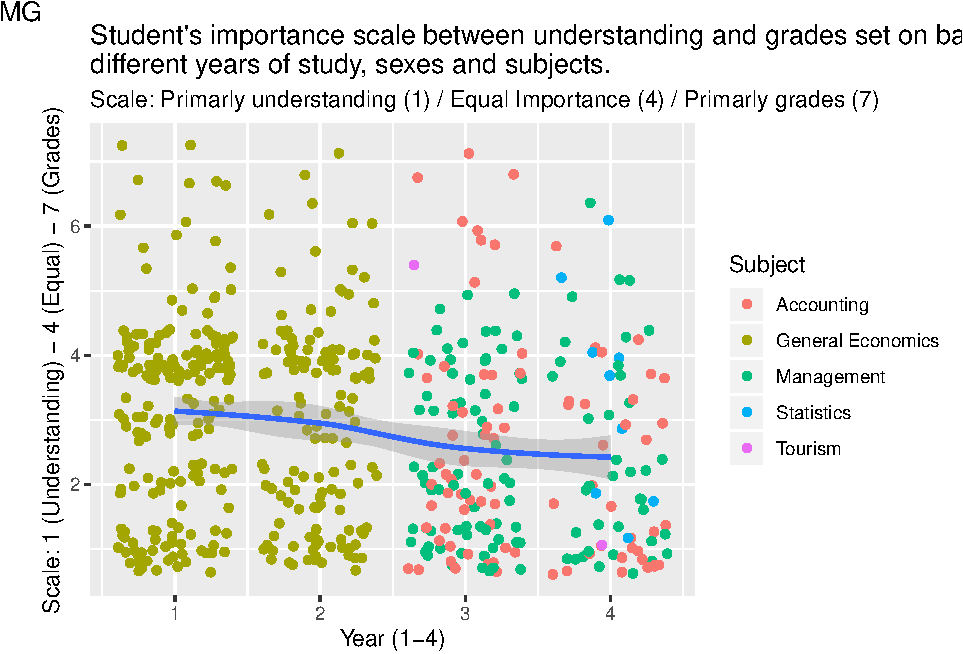
\includegraphics{StudentGoals_files/figure-latex/unnamed-chunk-13-1.pdf}

\begin{Shaded}
\begin{Highlighting}[]
\CommentTok{# m2}
\CommentTok{# Plot mean results of performance avoidance}
\CommentTok{# for all students with relation to student's year, sex and subject}
\CommentTok{# data}
\NormalTok{d <-}\StringTok{ }\KeywordTok{ggplot}\NormalTok{(}\DataTypeTok{data =}\NormalTok{ dat, }\KeywordTok{aes}\NormalTok{(year, mean_dat}\OperatorTok{$}\NormalTok{m2))}
\CommentTok{# mapping data (use "jitter" to improve the graph and avoid gridding)}
\NormalTok{l <-}\StringTok{ }\NormalTok{d }\OperatorTok{+}\StringTok{ }\KeywordTok{geom_jitter}\NormalTok{(}\KeywordTok{aes}\NormalTok{(}\DataTypeTok{colour =}\NormalTok{ sex, }\DataTypeTok{shape =}\NormalTok{ subject))}
\CommentTok{# smoothing}
\NormalTok{s <-}\StringTok{ }\NormalTok{l }\OperatorTok{+}\StringTok{ }\KeywordTok{geom_smooth}\NormalTok{(}\DataTypeTok{method =}\NormalTok{ loess, }\DataTypeTok{formula =}\NormalTok{ y }\OperatorTok{~}\StringTok{ }\KeywordTok{log}\NormalTok{(x), }\DataTypeTok{se =} \OtherTok{TRUE}\NormalTok{)}
\CommentTok{# adding theme}
\NormalTok{t <-}\StringTok{ }\NormalTok{s }\OperatorTok{+}\StringTok{ }\KeywordTok{theme_dark}\NormalTok{()}
\CommentTok{# adding colouring}
\NormalTok{c <-}\StringTok{ }\NormalTok{t }\OperatorTok{+}\StringTok{ }\KeywordTok{scale_colour_brewer}\NormalTok{(}\DataTypeTok{palette =} \StringTok{"Pastel1"}\NormalTok{)}
\CommentTok{# adding labels}
\NormalTok{c }\OperatorTok{+}\StringTok{ }\KeywordTok{labs}\NormalTok{(}
  \DataTypeTok{title =} \StringTok{"Students' grade-orientation focus set on basis of:}
\StringTok{different years of study, sexes and subjects."}\NormalTok{,}
  \DataTypeTok{subtitle =} \StringTok{"How motivated are students by fear of performing poorly?"}\NormalTok{,}
  \DataTypeTok{caption =} \StringTok{"Data source: Elliot, A. J. and McGregor, H. A. (2001)"}\NormalTok{,}
  \DataTypeTok{x =} \StringTok{"Year: 1 - 4"}\NormalTok{,}
  \DataTypeTok{y =} \StringTok{"Answer: 1 (Low) - 7 (High)"}\NormalTok{,}
  \DataTypeTok{colour =} \StringTok{"Sex"}\NormalTok{,}
  \DataTypeTok{shape =} \StringTok{"Subject"}
\NormalTok{)}
\end{Highlighting}
\end{Shaded}

\begin{verbatim}
## Warning in simpleLoess(y, x, w, span, degree = degree, parametric =
## parametric, : pseudoinverse used at -0.0069315
\end{verbatim}

\begin{verbatim}
## Warning in simpleLoess(y, x, w, span, degree = degree, parametric =
## parametric, : neighborhood radius 1.1055
\end{verbatim}

\begin{verbatim}
## Warning in simpleLoess(y, x, w, span, degree = degree, parametric =
## parametric, : reciprocal condition number 2.8144e-16
\end{verbatim}

\begin{verbatim}
## Warning in simpleLoess(y, x, w, span, degree = degree, parametric =
## parametric, : There are other near singularities as well. 0.48045
\end{verbatim}

\begin{verbatim}
## Warning in predLoess(object$y, object$x, newx = if
## (is.null(newdata)) object$x else if (is.data.frame(newdata))
## as.matrix(model.frame(delete.response(terms(object)), : pseudoinverse used
## at -0.0069315
\end{verbatim}

\begin{verbatim}
## Warning in predLoess(object$y, object$x, newx = if
## (is.null(newdata)) object$x else if (is.data.frame(newdata))
## as.matrix(model.frame(delete.response(terms(object)), : neighborhood radius
## 1.1055
\end{verbatim}

\begin{verbatim}
## Warning in predLoess(object$y, object$x, newx = if
## (is.null(newdata)) object$x else if (is.data.frame(newdata))
## as.matrix(model.frame(delete.response(terms(object)), : reciprocal
## condition number 2.8144e-16
\end{verbatim}

\begin{verbatim}
## Warning in predLoess(object$y, object$x, newx = if
## (is.null(newdata)) object$x else if (is.data.frame(newdata))
## as.matrix(model.frame(delete.response(terms(object)), : There are other
## near singularities as well. 0.48045
\end{verbatim}

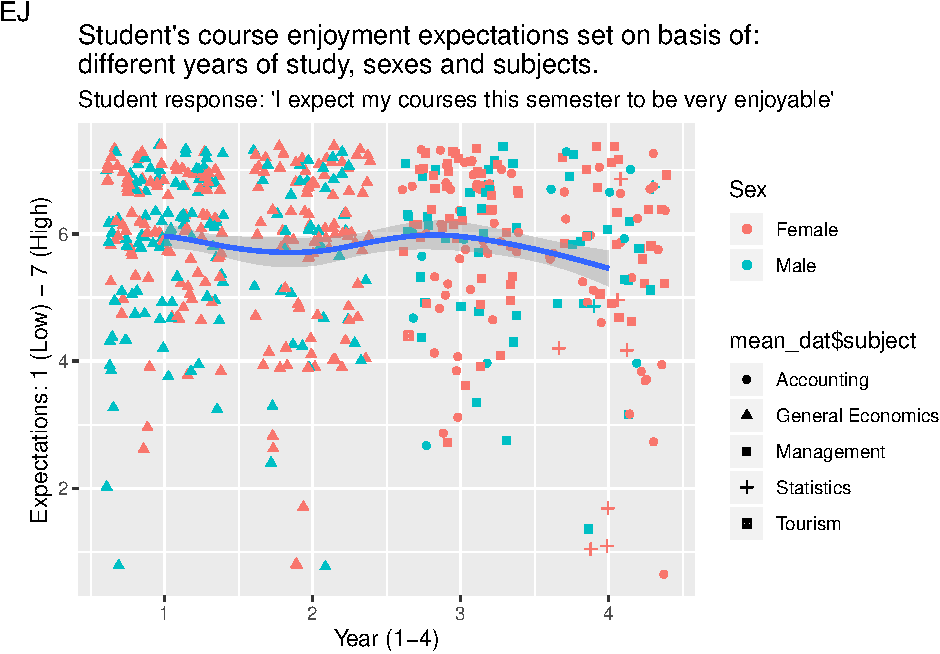
\includegraphics{StudentGoals_files/figure-latex/unnamed-chunk-14-1.pdf}

\begin{Shaded}
\begin{Highlighting}[]
\CommentTok{# m3}
\CommentTok{# Plot mean results of mastery approach questions}
\CommentTok{# for all students with relation to student's year, sex and subject}
\CommentTok{# data}
\NormalTok{d <-}\StringTok{ }\KeywordTok{ggplot}\NormalTok{(}\DataTypeTok{data =}\NormalTok{ dat, }\KeywordTok{aes}\NormalTok{(year, mean_dat}\OperatorTok{$}\NormalTok{m3))}
\CommentTok{# mapping data (use "jitter" to improve the graph and avoid gridding)}
\NormalTok{l <-}\StringTok{ }\NormalTok{d }\OperatorTok{+}\StringTok{ }\KeywordTok{geom_jitter}\NormalTok{(}\KeywordTok{aes}\NormalTok{(}\DataTypeTok{colour =}\NormalTok{ sex, }\DataTypeTok{shape =}\NormalTok{ subject))}
\CommentTok{# smoothing}
\NormalTok{s <-}\StringTok{ }\NormalTok{l }\OperatorTok{+}\StringTok{ }\KeywordTok{geom_smooth}\NormalTok{(}\DataTypeTok{method =}\NormalTok{ stats}\OperatorTok{::}\NormalTok{loess, }\DataTypeTok{formula =}\NormalTok{ y }\OperatorTok{~}\StringTok{ }\KeywordTok{log}\NormalTok{(x), }\DataTypeTok{se =} \OtherTok{TRUE}\NormalTok{)}
\CommentTok{# adding theme}
\NormalTok{t <-}\StringTok{ }\NormalTok{s }\OperatorTok{+}\StringTok{ }\KeywordTok{theme_dark}\NormalTok{()}
\CommentTok{# adding colouring}
\NormalTok{c <-}\StringTok{ }\NormalTok{t }\OperatorTok{+}\StringTok{ }\KeywordTok{scale_colour_brewer}\NormalTok{(}\DataTypeTok{palette =} \StringTok{"Pastel1"}\NormalTok{)}
\CommentTok{# adding labels}
\NormalTok{c }\OperatorTok{+}\StringTok{ }\KeywordTok{labs}\NormalTok{(}
  \DataTypeTok{title =} \StringTok{"Students' focus on understanding set on basis of:}
\StringTok{different years of study, sexes and subjects."}\NormalTok{,}
  \DataTypeTok{subtitle =} \StringTok{"Prevalence of mastery approach."}\NormalTok{,}
  \DataTypeTok{caption =} \StringTok{"Data source: Elliot, A. J. and McGregor, H. A. (2001)"}\NormalTok{,}
  \DataTypeTok{x =} \StringTok{"Year: 1 - 4"}\NormalTok{,}
  \DataTypeTok{y =} \StringTok{"Answer: 1 (Low) - 7 (High)"}\NormalTok{,}
  \DataTypeTok{colour =} \StringTok{"Sex"}\NormalTok{,}
  \DataTypeTok{shape =} \StringTok{"Subject"}
\NormalTok{)}
\end{Highlighting}
\end{Shaded}

\begin{verbatim}
## Warning in simpleLoess(y, x, w, span, degree = degree, parametric =
## parametric, : pseudoinverse used at -0.0069315
\end{verbatim}

\begin{verbatim}
## Warning in simpleLoess(y, x, w, span, degree = degree, parametric =
## parametric, : neighborhood radius 1.1055
\end{verbatim}

\begin{verbatim}
## Warning in simpleLoess(y, x, w, span, degree = degree, parametric =
## parametric, : reciprocal condition number 2.8144e-16
\end{verbatim}

\begin{verbatim}
## Warning in simpleLoess(y, x, w, span, degree = degree, parametric =
## parametric, : There are other near singularities as well. 0.48045
\end{verbatim}

\begin{verbatim}
## Warning in predLoess(object$y, object$x, newx = if
## (is.null(newdata)) object$x else if (is.data.frame(newdata))
## as.matrix(model.frame(delete.response(terms(object)), : pseudoinverse used
## at -0.0069315
\end{verbatim}

\begin{verbatim}
## Warning in predLoess(object$y, object$x, newx = if
## (is.null(newdata)) object$x else if (is.data.frame(newdata))
## as.matrix(model.frame(delete.response(terms(object)), : neighborhood radius
## 1.1055
\end{verbatim}

\begin{verbatim}
## Warning in predLoess(object$y, object$x, newx = if
## (is.null(newdata)) object$x else if (is.data.frame(newdata))
## as.matrix(model.frame(delete.response(terms(object)), : reciprocal
## condition number 2.8144e-16
\end{verbatim}

\begin{verbatim}
## Warning in predLoess(object$y, object$x, newx = if
## (is.null(newdata)) object$x else if (is.data.frame(newdata))
## as.matrix(model.frame(delete.response(terms(object)), : There are other
## near singularities as well. 0.48045
\end{verbatim}

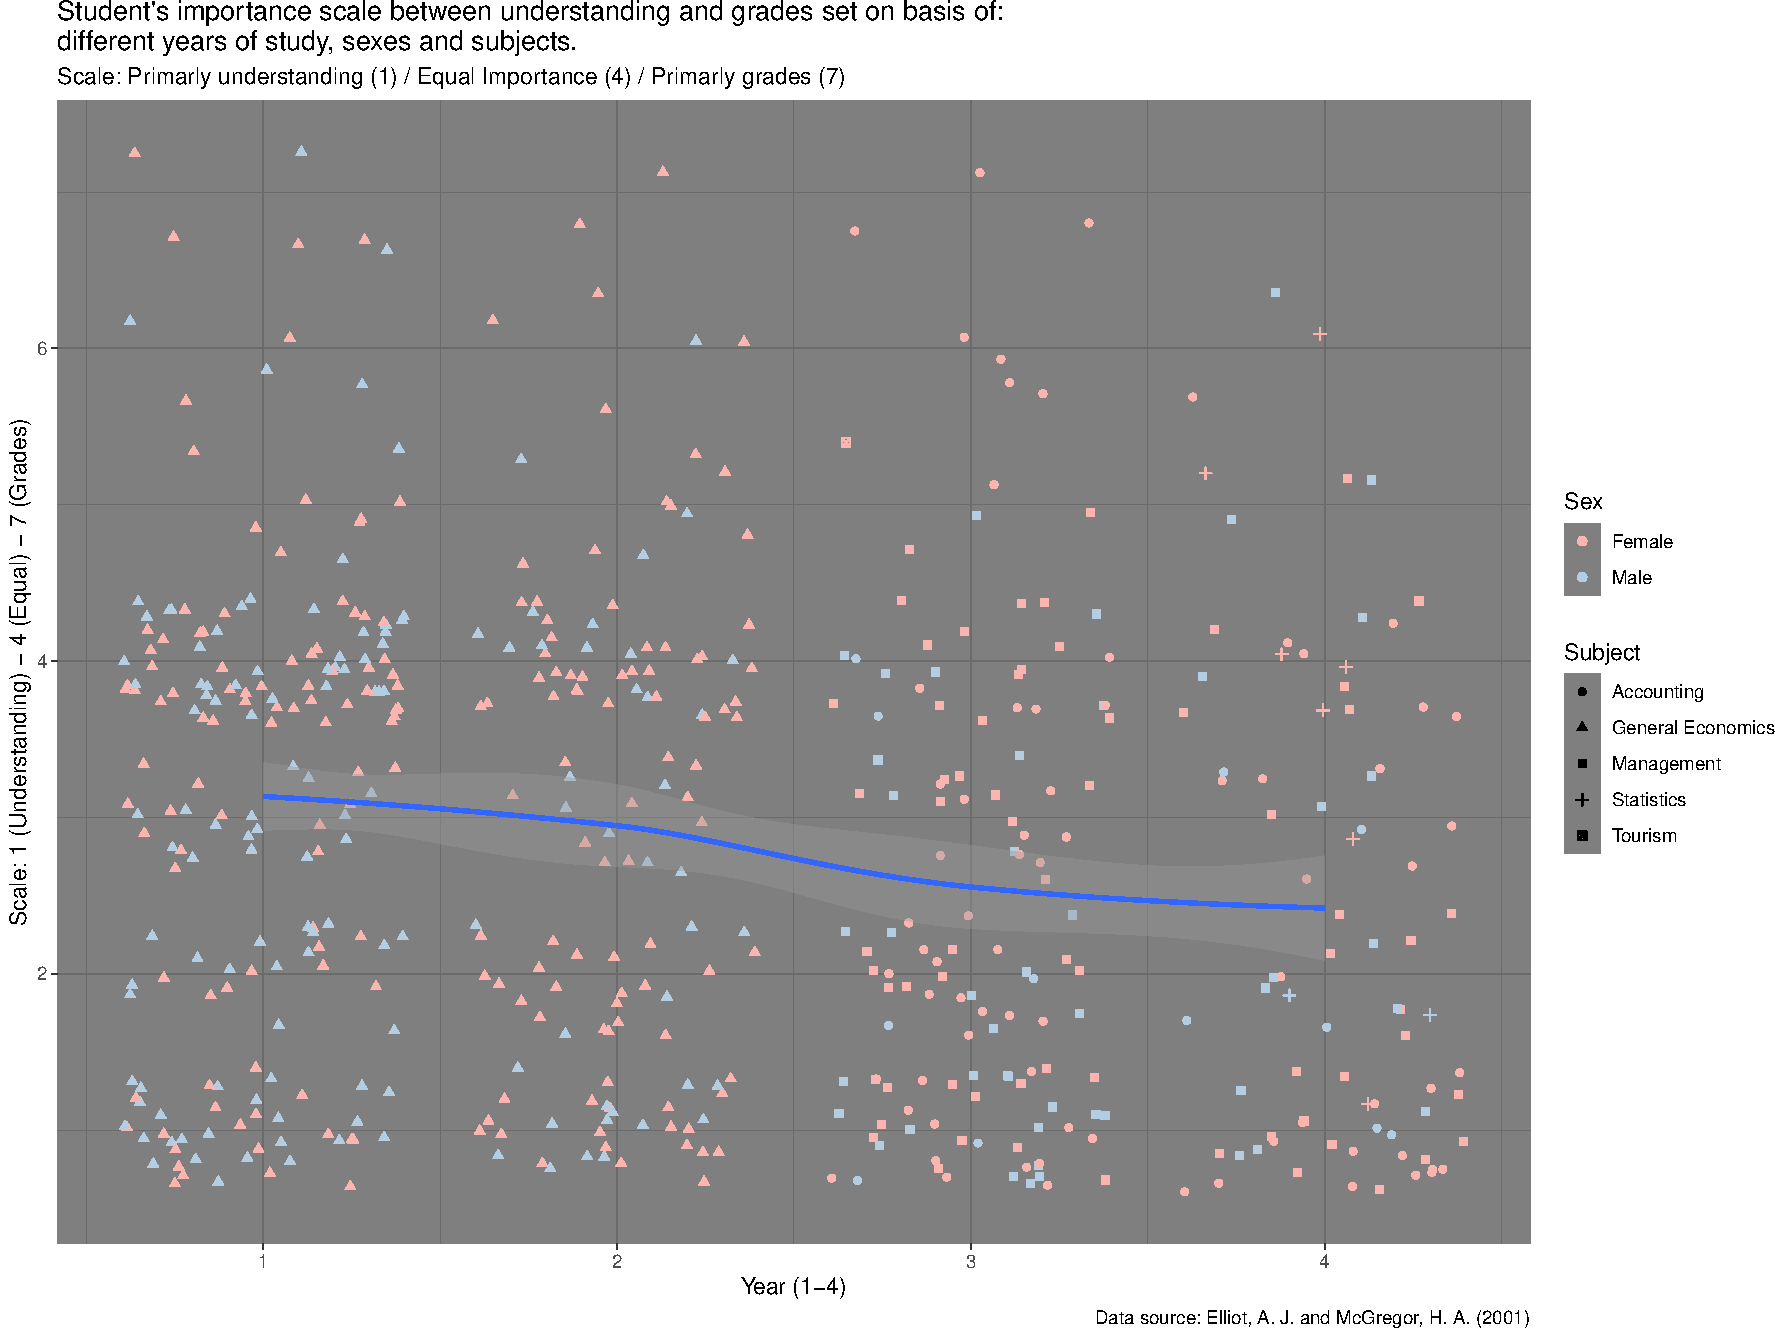
\includegraphics{StudentGoals_files/figure-latex/unnamed-chunk-15-1.pdf}

\begin{Shaded}
\begin{Highlighting}[]
\CommentTok{# m4}
\CommentTok{# Plot mean results of mastery avoidance questions}
\CommentTok{# for all students with relation to student's year, sex and subject}
\CommentTok{# data}
\NormalTok{d <-}\StringTok{ }\KeywordTok{ggplot}\NormalTok{(}\DataTypeTok{data =}\NormalTok{ dat, }\KeywordTok{aes}\NormalTok{(year, mean_dat}\OperatorTok{$}\NormalTok{m4))}
\CommentTok{# mapping data (use "jitter" to improve the graph and avoid gridding)}
\NormalTok{l <-}\StringTok{ }\NormalTok{d }\OperatorTok{+}\StringTok{ }\KeywordTok{geom_jitter}\NormalTok{(}\KeywordTok{aes}\NormalTok{(}\DataTypeTok{colour =}\NormalTok{ sex, }\DataTypeTok{shape =}\NormalTok{ subject))}
\CommentTok{# smoothing}
\NormalTok{s <-}\StringTok{ }\NormalTok{l }\OperatorTok{+}\StringTok{ }\KeywordTok{geom_smooth}\NormalTok{(}\DataTypeTok{method =}\NormalTok{ stats}\OperatorTok{::}\NormalTok{loess, }\DataTypeTok{formula =}\NormalTok{ y }\OperatorTok{~}\StringTok{ }\KeywordTok{log}\NormalTok{(x), }\DataTypeTok{se =} \OtherTok{TRUE}\NormalTok{)}
\CommentTok{# adding theme}
\NormalTok{t <-}\StringTok{ }\NormalTok{s }\OperatorTok{+}\StringTok{ }\KeywordTok{theme_dark}\NormalTok{()}
\CommentTok{# adding colouring}
\NormalTok{c <-}\StringTok{ }\NormalTok{t }\OperatorTok{+}\StringTok{ }\KeywordTok{scale_colour_brewer}\NormalTok{(}\DataTypeTok{palette =} \StringTok{"Pastel1"}\NormalTok{)}
\CommentTok{# adding labels}
\NormalTok{c }\OperatorTok{+}\StringTok{ }\KeywordTok{labs}\NormalTok{(}
  \DataTypeTok{title =} \StringTok{"Students' focus on understanding set on basis of:}
\StringTok{different years of study, sexes and subjects."}\NormalTok{,}
  \DataTypeTok{subtitle =} \StringTok{"Students' fear of not mastering the course."}\NormalTok{,}
  \DataTypeTok{caption =} \StringTok{"Data source: Elliot, A. J. and McGregor, H. A. (2001)"}\NormalTok{,}
  \DataTypeTok{x =} \StringTok{"Year: 1 - 4"}\NormalTok{,}
  \DataTypeTok{y =} \StringTok{"Answer: 1 (Low) - 7 (High)"}\NormalTok{,}
  \DataTypeTok{colour =} \StringTok{"Sex"}\NormalTok{,}
  \DataTypeTok{shape =} \StringTok{"Subject"}
\NormalTok{)}
\end{Highlighting}
\end{Shaded}

\begin{verbatim}
## Warning in simpleLoess(y, x, w, span, degree = degree, parametric =
## parametric, : pseudoinverse used at -0.0069315
\end{verbatim}

\begin{verbatim}
## Warning in simpleLoess(y, x, w, span, degree = degree, parametric =
## parametric, : neighborhood radius 1.1055
\end{verbatim}

\begin{verbatim}
## Warning in simpleLoess(y, x, w, span, degree = degree, parametric =
## parametric, : reciprocal condition number 2.8144e-16
\end{verbatim}

\begin{verbatim}
## Warning in simpleLoess(y, x, w, span, degree = degree, parametric =
## parametric, : There are other near singularities as well. 0.48045
\end{verbatim}

\begin{verbatim}
## Warning in predLoess(object$y, object$x, newx = if
## (is.null(newdata)) object$x else if (is.data.frame(newdata))
## as.matrix(model.frame(delete.response(terms(object)), : pseudoinverse used
## at -0.0069315
\end{verbatim}

\begin{verbatim}
## Warning in predLoess(object$y, object$x, newx = if
## (is.null(newdata)) object$x else if (is.data.frame(newdata))
## as.matrix(model.frame(delete.response(terms(object)), : neighborhood radius
## 1.1055
\end{verbatim}

\begin{verbatim}
## Warning in predLoess(object$y, object$x, newx = if
## (is.null(newdata)) object$x else if (is.data.frame(newdata))
## as.matrix(model.frame(delete.response(terms(object)), : reciprocal
## condition number 2.8144e-16
\end{verbatim}

\begin{verbatim}
## Warning in predLoess(object$y, object$x, newx = if
## (is.null(newdata)) object$x else if (is.data.frame(newdata))
## as.matrix(model.frame(delete.response(terms(object)), : There are other
## near singularities as well. 0.48045
\end{verbatim}

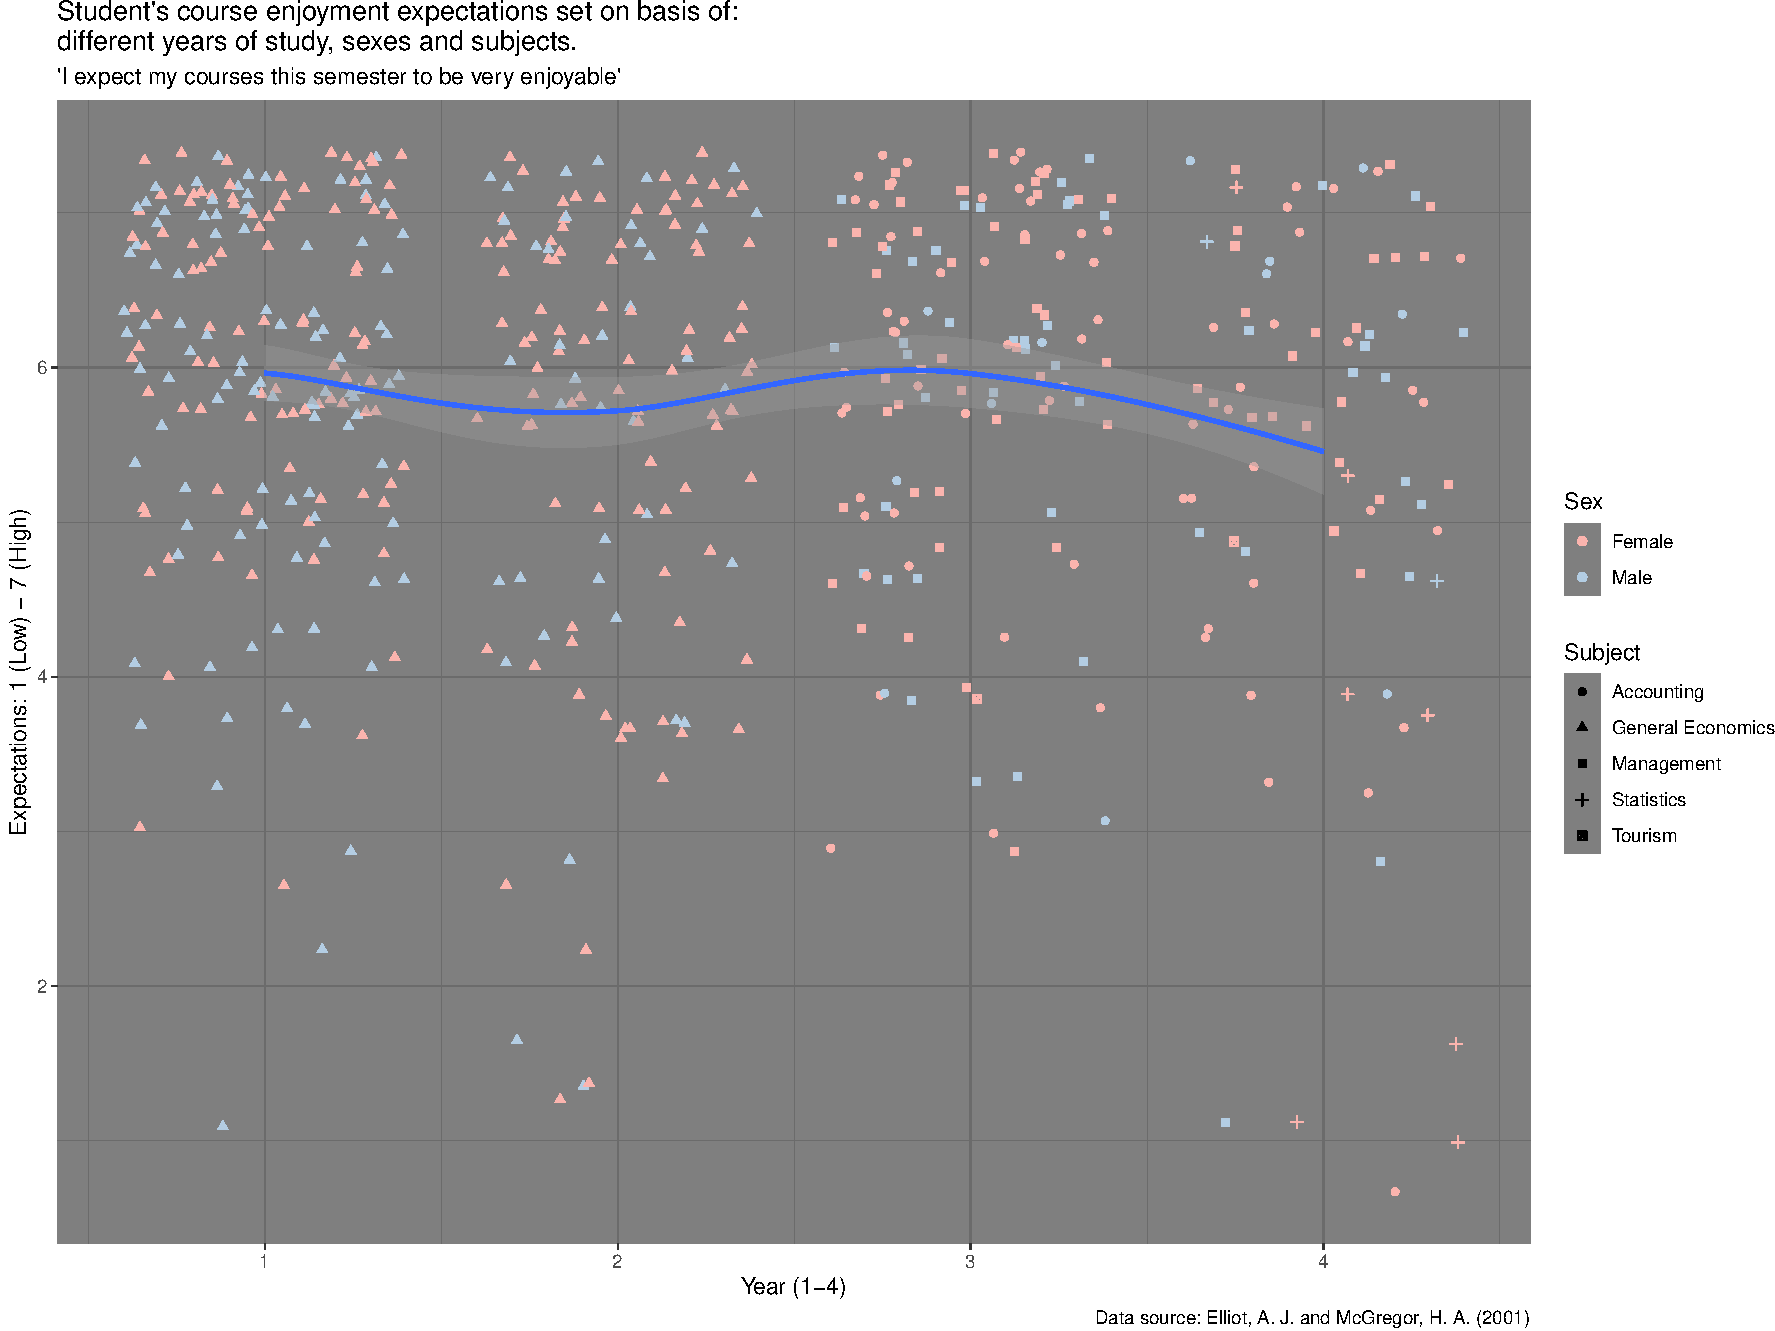
\includegraphics{StudentGoals_files/figure-latex/unnamed-chunk-16-1.pdf}

\begin{Shaded}
\begin{Highlighting}[]
\CommentTok{# interest}
\CommentTok{# Plot mean results of course interestedness expectations questions}
\CommentTok{# for all students with relation to student's year, sex and subject}
\CommentTok{# data}
\NormalTok{d <-}\StringTok{ }\KeywordTok{ggplot}\NormalTok{(}\DataTypeTok{data =}\NormalTok{ dat, }\KeywordTok{aes}\NormalTok{(year, mean_dat}\OperatorTok{$}\NormalTok{m_interest))}
\CommentTok{# mapping data (use "jitter" to improve the graph and avoid gridding)}
\NormalTok{l <-}\StringTok{ }\NormalTok{d }\OperatorTok{+}\StringTok{ }\KeywordTok{geom_jitter}\NormalTok{(}\KeywordTok{aes}\NormalTok{(}\DataTypeTok{colour =}\NormalTok{ sex, }\DataTypeTok{shape =}\NormalTok{ subject))}
\CommentTok{# smoothing}
\NormalTok{s <-}\StringTok{ }\NormalTok{l }\OperatorTok{+}\StringTok{ }\KeywordTok{geom_smooth}\NormalTok{(}\DataTypeTok{method =}\NormalTok{ stats}\OperatorTok{::}\NormalTok{loess, }\DataTypeTok{formula =}\NormalTok{ y }\OperatorTok{~}\StringTok{ }\KeywordTok{log}\NormalTok{(x), }\DataTypeTok{se =} \OtherTok{TRUE}\NormalTok{)}
\CommentTok{# adding theme}
\NormalTok{t <-}\StringTok{ }\NormalTok{s }\OperatorTok{+}\StringTok{ }\KeywordTok{theme_dark}\NormalTok{()}
\CommentTok{# adding colouring}
\NormalTok{c <-}\StringTok{ }\NormalTok{t }\OperatorTok{+}\StringTok{ }\KeywordTok{scale_colour_brewer}\NormalTok{(}\DataTypeTok{palette =} \StringTok{"Pastel1"}\NormalTok{)}
\CommentTok{# adding labels}
\NormalTok{c }\OperatorTok{+}\StringTok{ }\KeywordTok{labs}\NormalTok{(}
  \DataTypeTok{title =} \StringTok{"Students' course interestedness expectations set on basis of:}
\StringTok{different years of study, sexes and subjects."}\NormalTok{,}
  \DataTypeTok{subtitle =} \StringTok{"}\CharTok{\textbackslash{}'}\StringTok{I expect my courses this semester to be very interesting}\CharTok{\textbackslash{}'}\StringTok{"}\NormalTok{,}
  \DataTypeTok{caption =} \StringTok{"Data source: Elliot, A. J. and McGregor, H. A. (2001)"}\NormalTok{,}
  \DataTypeTok{x =} \StringTok{"Year (1-4)"}\NormalTok{,}
  \DataTypeTok{y =} \StringTok{"Expectations: 1 (Low) - 7 (High)"}\NormalTok{,}
  \DataTypeTok{colour =} \StringTok{"Sex"}\NormalTok{,}
  \DataTypeTok{shape =} \StringTok{"Subject"}
\NormalTok{)}
\end{Highlighting}
\end{Shaded}

\begin{verbatim}
## Warning in simpleLoess(y, x, w, span, degree = degree, parametric =
## parametric, : pseudoinverse used at -0.0069315
\end{verbatim}

\begin{verbatim}
## Warning in simpleLoess(y, x, w, span, degree = degree, parametric =
## parametric, : neighborhood radius 1.1055
\end{verbatim}

\begin{verbatim}
## Warning in simpleLoess(y, x, w, span, degree = degree, parametric =
## parametric, : reciprocal condition number 2.8144e-16
\end{verbatim}

\begin{verbatim}
## Warning in simpleLoess(y, x, w, span, degree = degree, parametric =
## parametric, : There are other near singularities as well. 0.48045
\end{verbatim}

\begin{verbatim}
## Warning in predLoess(object$y, object$x, newx = if
## (is.null(newdata)) object$x else if (is.data.frame(newdata))
## as.matrix(model.frame(delete.response(terms(object)), : pseudoinverse used
## at -0.0069315
\end{verbatim}

\begin{verbatim}
## Warning in predLoess(object$y, object$x, newx = if
## (is.null(newdata)) object$x else if (is.data.frame(newdata))
## as.matrix(model.frame(delete.response(terms(object)), : neighborhood radius
## 1.1055
\end{verbatim}

\begin{verbatim}
## Warning in predLoess(object$y, object$x, newx = if
## (is.null(newdata)) object$x else if (is.data.frame(newdata))
## as.matrix(model.frame(delete.response(terms(object)), : reciprocal
## condition number 2.8144e-16
\end{verbatim}

\begin{verbatim}
## Warning in predLoess(object$y, object$x, newx = if
## (is.null(newdata)) object$x else if (is.data.frame(newdata))
## as.matrix(model.frame(delete.response(terms(object)), : There are other
## near singularities as well. 0.48045
\end{verbatim}

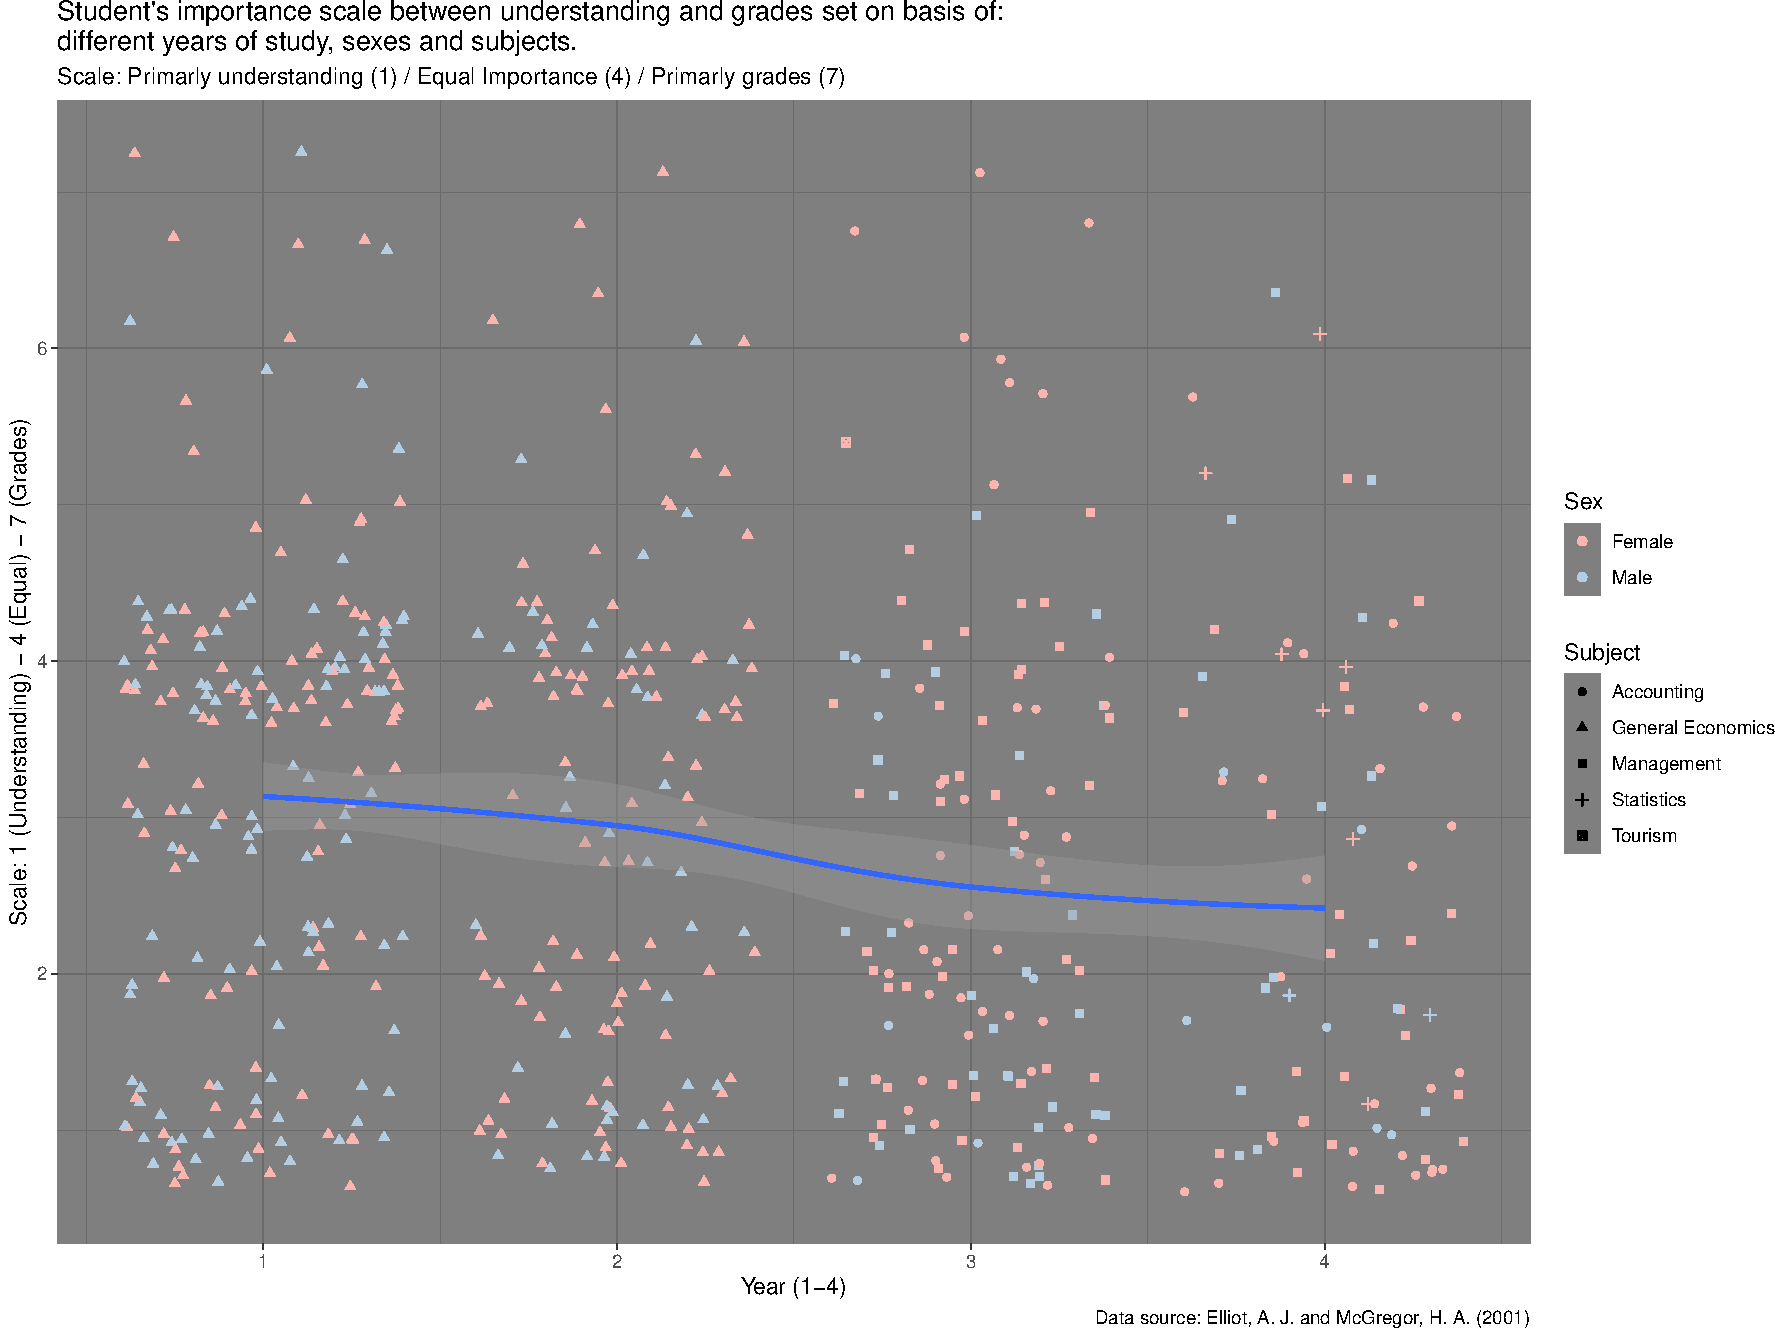
\includegraphics{StudentGoals_files/figure-latex/unnamed-chunk-17-1.pdf}

\begin{Shaded}
\begin{Highlighting}[]
\CommentTok{# chi-squared}
\NormalTok{chi_sqrt <-}\StringTok{ }\KeywordTok{ggplot}\NormalTok{(}\DataTypeTok{data =}\NormalTok{ dat, }\KeywordTok{aes}\NormalTok{(year, mean_dat}\OperatorTok{$}\NormalTok{m_interest)) }\OperatorTok{+}
\StringTok{  }\KeywordTok{stat_function}\NormalTok{(}\DataTypeTok{fun =}\NormalTok{ dchisq, }\DataTypeTok{args =} \KeywordTok{list}\NormalTok{(}\DataTypeTok{df =} \DecValTok{8}\NormalTok{))}
\NormalTok{chi_sqrt}
\end{Highlighting}
\end{Shaded}

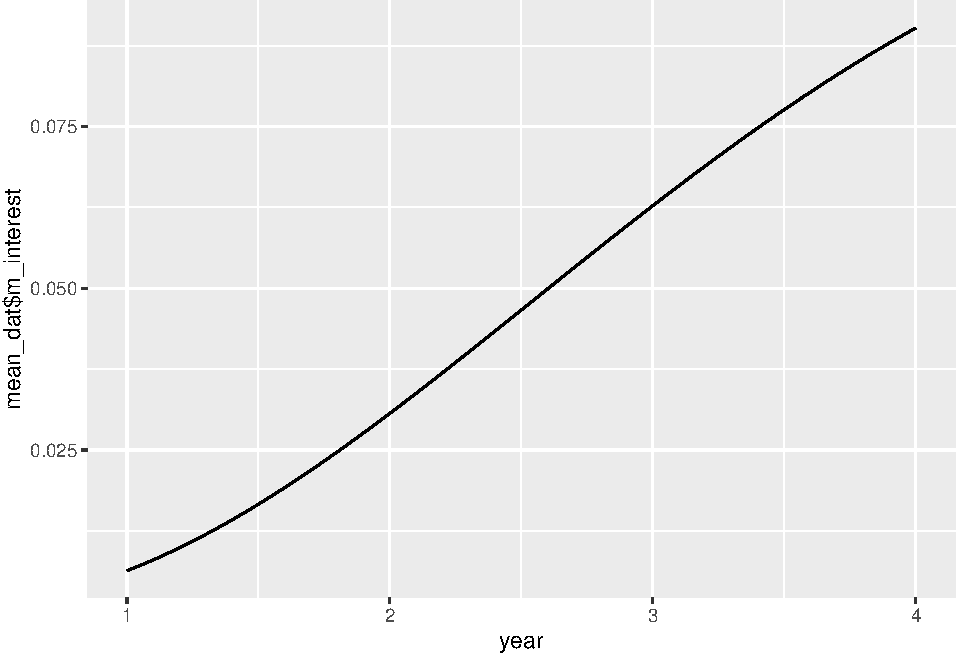
\includegraphics{StudentGoals_files/figure-latex/unnamed-chunk-17-2.pdf}

\begin{Shaded}
\begin{Highlighting}[]
\CommentTok{# enjoy}
\CommentTok{# Plot mean results of course enjoyment expectations questions }
\CommentTok{# for all students with relation to student's year, sex and subject}
\CommentTok{# data}
\NormalTok{d <-}\StringTok{ }\KeywordTok{ggplot}\NormalTok{(}\DataTypeTok{data =}\NormalTok{ dat, }\KeywordTok{aes}\NormalTok{(year, mean_dat}\OperatorTok{$}\NormalTok{m_enjoy))}
\CommentTok{# mapping data (use "jitter" to improve the graph and avoid gridding)}
\NormalTok{l <-}\StringTok{ }\NormalTok{d }\OperatorTok{+}\StringTok{ }\KeywordTok{geom_jitter}\NormalTok{(}\KeywordTok{aes}\NormalTok{(}\DataTypeTok{colour =}\NormalTok{ sex, }\DataTypeTok{shape =}\NormalTok{ subject))}
\CommentTok{# smoothing}
\NormalTok{s <-}\StringTok{ }\NormalTok{l }\OperatorTok{+}\StringTok{ }\KeywordTok{geom_smooth}\NormalTok{(}\DataTypeTok{method =}\NormalTok{ stats}\OperatorTok{::}\NormalTok{loess, }\DataTypeTok{formula =}\NormalTok{ y }\OperatorTok{~}\StringTok{ }\KeywordTok{log}\NormalTok{(x), }\DataTypeTok{se =} \OtherTok{TRUE}\NormalTok{)}
\CommentTok{# adding theme}
\NormalTok{t <-}\StringTok{ }\NormalTok{s }\OperatorTok{+}\StringTok{ }\KeywordTok{theme_dark}\NormalTok{()}
\CommentTok{# adding colouring}
\NormalTok{c <-}\StringTok{ }\NormalTok{t }\OperatorTok{+}\StringTok{ }\KeywordTok{scale_colour_brewer}\NormalTok{(}\DataTypeTok{palette =} \StringTok{"Pastel1"}\NormalTok{)}
\CommentTok{# adding labels}
\NormalTok{c }\OperatorTok{+}\StringTok{ }\KeywordTok{labs}\NormalTok{(}
  \DataTypeTok{title =} \StringTok{"Students' course enjoyment expectations set on basis of:}
\StringTok{different years of study, sexes and subjects."}\NormalTok{,}
  \DataTypeTok{subtitle =} \StringTok{"}\CharTok{\textbackslash{}'}\StringTok{I expect my courses this semester to be very enjoyable}\CharTok{\textbackslash{}'}\StringTok{"}\NormalTok{,}
  \DataTypeTok{caption =} \StringTok{"Data source: Elliot, A. J. and McGregor, H. A. (2001)"}\NormalTok{,}
  \DataTypeTok{x =} \StringTok{"Year (1-4)"}\NormalTok{,}
  \DataTypeTok{y =} \StringTok{"Expectations: 1 (Low) - 7 (High)"}\NormalTok{,}
  \DataTypeTok{colour =} \StringTok{"Sex"}\NormalTok{,}
  \DataTypeTok{shape =} \StringTok{"Subject"}
\NormalTok{)}
\end{Highlighting}
\end{Shaded}

\begin{verbatim}
## Warning in simpleLoess(y, x, w, span, degree = degree, parametric =
## parametric, : pseudoinverse used at -0.0069315
\end{verbatim}

\begin{verbatim}
## Warning in simpleLoess(y, x, w, span, degree = degree, parametric =
## parametric, : neighborhood radius 1.1055
\end{verbatim}

\begin{verbatim}
## Warning in simpleLoess(y, x, w, span, degree = degree, parametric =
## parametric, : reciprocal condition number 2.8144e-16
\end{verbatim}

\begin{verbatim}
## Warning in simpleLoess(y, x, w, span, degree = degree, parametric =
## parametric, : There are other near singularities as well. 0.48045
\end{verbatim}

\begin{verbatim}
## Warning in predLoess(object$y, object$x, newx = if
## (is.null(newdata)) object$x else if (is.data.frame(newdata))
## as.matrix(model.frame(delete.response(terms(object)), : pseudoinverse used
## at -0.0069315
\end{verbatim}

\begin{verbatim}
## Warning in predLoess(object$y, object$x, newx = if
## (is.null(newdata)) object$x else if (is.data.frame(newdata))
## as.matrix(model.frame(delete.response(terms(object)), : neighborhood radius
## 1.1055
\end{verbatim}

\begin{verbatim}
## Warning in predLoess(object$y, object$x, newx = if
## (is.null(newdata)) object$x else if (is.data.frame(newdata))
## as.matrix(model.frame(delete.response(terms(object)), : reciprocal
## condition number 2.8144e-16
\end{verbatim}

\begin{verbatim}
## Warning in predLoess(object$y, object$x, newx = if
## (is.null(newdata)) object$x else if (is.data.frame(newdata))
## as.matrix(model.frame(delete.response(terms(object)), : There are other
## near singularities as well. 0.48045
\end{verbatim}

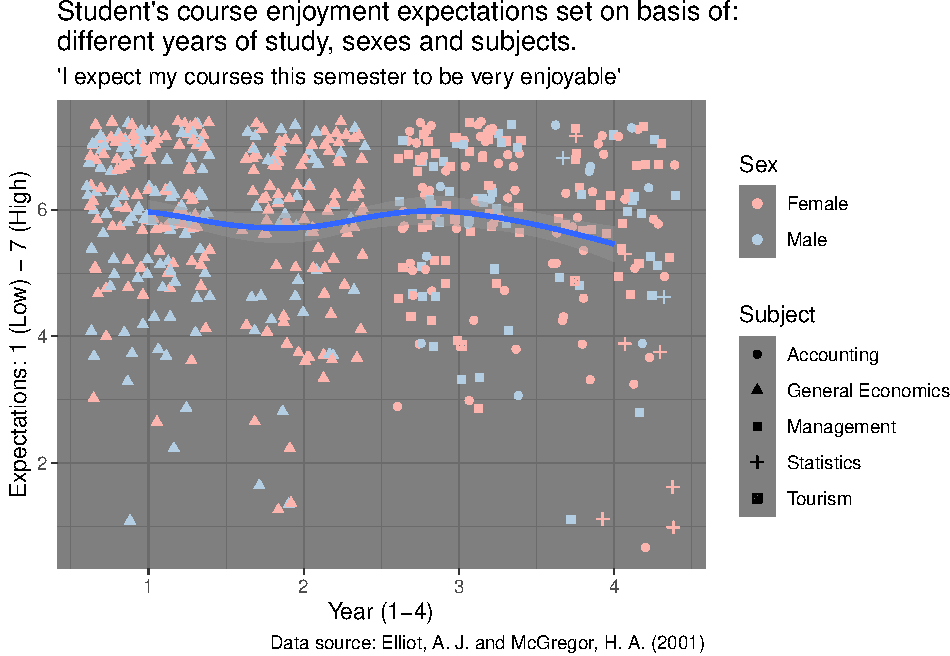
\includegraphics{StudentGoals_files/figure-latex/unnamed-chunk-18-1.pdf}

\begin{Shaded}
\begin{Highlighting}[]
\CommentTok{# mastgrad}
\CommentTok{# Plot mean results of (Primarly understanding/Equal Importance/Primarly grades)scale }
\CommentTok{# for all students with relation to student's year, sex and subject}
\CommentTok{# data}
\NormalTok{d <-}\StringTok{ }\KeywordTok{ggplot}\NormalTok{(}\DataTypeTok{data =}\NormalTok{ dat, }\KeywordTok{aes}\NormalTok{(year, mean_dat}\OperatorTok{$}\NormalTok{m_mastgrad))}
\CommentTok{# mapping data (use "jitter" to improve the graph and avoid gridding)}
\NormalTok{l <-}\StringTok{ }\NormalTok{d }\OperatorTok{+}\StringTok{ }\KeywordTok{geom_jitter}\NormalTok{(}\KeywordTok{aes}\NormalTok{(}\DataTypeTok{colour =}\NormalTok{ sex, }\DataTypeTok{shape =}\NormalTok{ subject))}
\CommentTok{# smoothing}
\NormalTok{s <-}\StringTok{ }\NormalTok{l }\OperatorTok{+}\StringTok{ }\KeywordTok{geom_smooth}\NormalTok{(}\DataTypeTok{method =}\NormalTok{ stats}\OperatorTok{::}\NormalTok{loess, }\DataTypeTok{formula =}\NormalTok{ y }\OperatorTok{~}\StringTok{ }\KeywordTok{log}\NormalTok{(x), }\DataTypeTok{se =} \OtherTok{TRUE}\NormalTok{)}
\CommentTok{# adding theme}
\NormalTok{t <-}\StringTok{ }\NormalTok{s }\OperatorTok{+}\StringTok{ }\KeywordTok{theme_dark}\NormalTok{()}
\CommentTok{# adding colouring}
\NormalTok{c <-}\StringTok{ }\NormalTok{t }\OperatorTok{+}\StringTok{ }\KeywordTok{scale_colour_brewer}\NormalTok{(}\DataTypeTok{palette =} \StringTok{"Pastel1"}\NormalTok{)}
\CommentTok{# adding labels}
\NormalTok{c }\OperatorTok{+}\StringTok{ }\KeywordTok{labs}\NormalTok{(}
  \DataTypeTok{title =} \StringTok{"Students' importance scale between understanding and grades set on basis of:}
\StringTok{different years of study, sexes and subjects."}\NormalTok{,}
  \DataTypeTok{subtitle =} \StringTok{"Scale: Primarly understanding (1) / Equal Importance (4) / Primarly grades (7)"}\NormalTok{,}
  \DataTypeTok{caption =} \StringTok{"Data source: Elliot, A. J. and McGregor, H. A. (2001)"}\NormalTok{,}
  \DataTypeTok{x =} \StringTok{"Year (1-4)"}\NormalTok{,}
  \DataTypeTok{y =} \StringTok{"Scale: 1 (Understanding) - 4 (Equal) - 7 (Grades)"}\NormalTok{,}
  \DataTypeTok{colour =} \StringTok{"Sex"}\NormalTok{,}
  \DataTypeTok{shape =} \StringTok{"Subject"}
\NormalTok{)}
\end{Highlighting}
\end{Shaded}

\begin{verbatim}
## Warning in simpleLoess(y, x, w, span, degree = degree, parametric =
## parametric, : pseudoinverse used at -0.0069315
\end{verbatim}

\begin{verbatim}
## Warning in simpleLoess(y, x, w, span, degree = degree, parametric =
## parametric, : neighborhood radius 1.1055
\end{verbatim}

\begin{verbatim}
## Warning in simpleLoess(y, x, w, span, degree = degree, parametric =
## parametric, : reciprocal condition number 2.8144e-16
\end{verbatim}

\begin{verbatim}
## Warning in simpleLoess(y, x, w, span, degree = degree, parametric =
## parametric, : There are other near singularities as well. 0.48045
\end{verbatim}

\begin{verbatim}
## Warning in predLoess(object$y, object$x, newx = if
## (is.null(newdata)) object$x else if (is.data.frame(newdata))
## as.matrix(model.frame(delete.response(terms(object)), : pseudoinverse used
## at -0.0069315
\end{verbatim}

\begin{verbatim}
## Warning in predLoess(object$y, object$x, newx = if
## (is.null(newdata)) object$x else if (is.data.frame(newdata))
## as.matrix(model.frame(delete.response(terms(object)), : neighborhood radius
## 1.1055
\end{verbatim}

\begin{verbatim}
## Warning in predLoess(object$y, object$x, newx = if
## (is.null(newdata)) object$x else if (is.data.frame(newdata))
## as.matrix(model.frame(delete.response(terms(object)), : reciprocal
## condition number 2.8144e-16
\end{verbatim}

\begin{verbatim}
## Warning in predLoess(object$y, object$x, newx = if
## (is.null(newdata)) object$x else if (is.data.frame(newdata))
## as.matrix(model.frame(delete.response(terms(object)), : There are other
## near singularities as well. 0.48045
\end{verbatim}

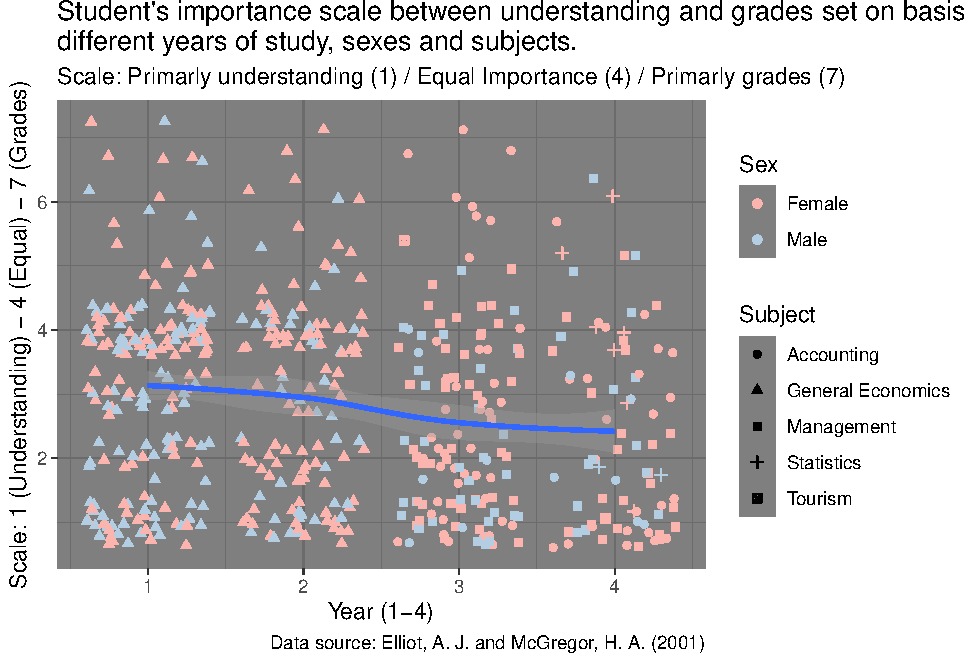
\includegraphics{StudentGoals_files/figure-latex/unnamed-chunk-19-1.pdf}

\begin{Shaded}
\begin{Highlighting}[]
\CommentTok{## CLASSIFICATION ###################################################}
\CommentTok{# dat_tibble %>%}
\CommentTok{#   head() %>%}
\CommentTok{#   knitr::kable()}

\CommentTok{# get only answers that are greater or equal to 5}
\NormalTok{dat_tibble_m1 <-}\StringTok{ }\KeywordTok{filter}\NormalTok{(dat_tibble, m1 }\OperatorTok{>=}\StringTok{ }\DecValTok{5}\NormalTok{)}

\NormalTok{n_m1 <-}\StringTok{ }\KeywordTok{tally}\NormalTok{(dat_tibble_m1) }\CommentTok{# 212}
\NormalTok{beta <-}\StringTok{ }\NormalTok{n_m1 }\OperatorTok{/}\StringTok{ }\NormalTok{n }\CommentTok{# 0.3392}

\NormalTok{ci <-}\StringTok{ }\NormalTok{beta }\OperatorTok{*}\StringTok{ }\NormalTok{((}\DecValTok{1} \OperatorTok{-}\StringTok{ }\NormalTok{beta)}\OperatorTok{/}\NormalTok{(n)) }\CommentTok{# 0.0003586294}
\NormalTok{ci_sqrt <-}\StringTok{ }\KeywordTok{sqrt}\NormalTok{(ci) }\CommentTok{# 0.0189}
\NormalTok{ci_margin_error <-}\StringTok{ }\NormalTok{ci_sqrt }\OperatorTok{*}\StringTok{ }\FloatTok{1.96} \CommentTok{# 0.0371 or 3.71% }

\CommentTok{# Our 95% confidence interval for the percentage of times we will get a student with a mean of}
\CommentTok{# 5 or above for the set of m1 questions is 0.3392 (or 34%), plus or minus 0.03711 (or 3.7%).}
\CommentTok{# The lower end of the interval is 0.3392 - 0.03711 which is:}
\NormalTok{lower_end_of_interval <-}\StringTok{ }\NormalTok{beta }\OperatorTok{-}\StringTok{ }\NormalTok{ci_margin_error }\CommentTok{# 0.3020825 or 30%}
\CommentTok{# The upper end of the interval is 0.3392}
\NormalTok{upper_end_of_interval <-}\StringTok{ }\NormalTok{beta }\OperatorTok{+}\StringTok{ }\NormalTok{ci_margin_error }\CommentTok{# 0.3763175 or 37%}

\CommentTok{# To interpret these results we could say that with 95% confidence the percentage of the times}
\CommentTok{# we should expect to find a student with a mean score of 5 or above to m1 is somewhere}
\CommentTok{# between 30% and 37%, based on our sample.}
\CommentTok{#####################################################################}
\end{Highlighting}
\end{Shaded}


\end{document}
